%% 
%% Copyright 2019-2020 Elsevier Ltd
%% 
%% This file is part of the 'CAS Bundle'.
%% --------------------------------------
%% 
%% It may be distributed under the conditions of the LaTeX Project Public
%% License, either version 1.2 of this license or (at your option) any
%% later version.  The latest version of this license is in
%%    http://www.latex-project.org/lppl.txt
%% and version 1.2 or later is part of all distributions of LaTeX
%% version 1999/12/01 or later.
%% 
%% The list of all files belonging to the 'CAS Bundle' is
%% given in the file `manifest.txt'.
%% 
%% Template article for cas-sc documentclass for 
%% single column output.

%\documentclass[a4paper,fleqn,longmktitle]{cas-sc}
\documentclass[a4paper,fleqn]{cas-sc}

%\usepackage[numbers]{natbib}
%\usepackage[authoryear]{natbib}
\usepackage{natbib}
\usepackage[textsize=small]{todonotes}
\usepackage{float}

\usepackage{graphicx}
\usepackage[center]{caption}
%%%%%%%%%%%%%% 	SYMBOLS		%%%%%%%%%%%%%%%%%
%                                    		%
%	Define all abstract set, variable,		%
%	function, and other generic symbols   	%
%                               			% %                              				%
%%%%%%%%%%%%%%%%%%%%%%%%%%%%%%%%%%%%%%%%%%%%%
\newtheorem{ass}{Assumption}
\newcommand{\assumption}[2]{
	\begin{ass}{(\textit{#1})}
		#2
	\end{ass}
}

\newcommand{\probability}[1]{
	P(#1)
}
\newcommand{\varSymbol}[3]{
\ifx \\#2\\
	\ifx \\#3\\ \lowercase{#1}
	\else
	\lowercase{#1}^{#3}
	\fi
\else
	\ifx \\#3\\ \lowercase{#1}_{#2}
	\else
		\lowercase{#1}_{#2}^{#3}
	\fi
\fi
}

\newcommand{\optimalVarSymbol}[3]
{
	\ifx\\#2\\
	\ifx\\#3\\ \optimal{\lowercase{#1}}
	\else
	\optimal{\lowercase{#1}}\textsuperscript{#3}
	\fi
	\else
	\ifx\\#3\\ \optimal{\lowercase{#1}}\textsubscript{#2}
	\else
	\optimal{\lowercase{#1}}\textsubscript{#2}\textsuperscript{#3}
	\fi
	\fi
}

\newcommand{\specialSetSymbol}[3]
{
	\ifx\\#2\\ \ifx\\#3\\  \overline{\uppercase{#1}}
	\else
	 \overline{\uppercase{#1}}\textsuperscript{#3}
	\fi
	\else
	\ifx\\#3\\  \overline{\uppercase{#1}}\textsubscript{#2}
	\else
	 \overline{\uppercase{#1}}\textsubscript{#2}\textsuperscript{#3}
	\fi
	\fi
}

\newcommand{\optimalSetSymbol}[3]
{
	\ifx\\#2\\ \ifx\\#3\\ \optimal{\uppercase{#1}}
	\else
	\optimal{\uppercase{#1}}\textsuperscript{#3}
	\fi
	\else
	\ifx\\#3\\ \optimal{\uppercase{#1}}\textsubscript{#2}
	\else
	\optimal{\uppercase{#1}}\textsubscript{#2}\textsuperscript{#3}
	\fi
	\fi
}

\newcommand{\estimatedOptimalVarSymbol}[3]
{
	\ifx\\#2\\
	\ifx\\#3\\ \optimal{\widetilde{\lowercase{#1}}}
	\else
	\optimal{\widetilde{\lowercase{#1}}}\textsuperscript{#3}
	\fi
	\else
	\ifx\\#3\\ \optimal{\widetilde{\lowercase{#1}}}\textsubscript{#2}
	\else
	\optimal{\widetilde{\lowercase{#1}}}\textsubscript{#2}\textsuperscript{#3}
	\fi
	\fi
}

\newcommand{\estimatedOptimalSetSymbol}[3]
{
	\ifx\\#2\\
	\ifx\\#3\\ \optimal{\widetilde{\uppercase{#1}}}
	\else \optimal{\widetilde{\uppercase{#1}}}\textsuperscript{#3}
	\fi
	\else \ifx\\#3\\ \optimal{\widetilde{\uppercase{#1}}}\textsubscript{#2}
	\else \optimal{\widetilde{\uppercase{#1}}}\textsubscript{#2}\textsuperscript{#3}
	\fi
	\fi
}



%%%%%%%%%% FUNCTIONS %%%%%%%%%%

\newcommand{\functionSymbol}[1]{\lowercase{#1}}
\newcommand{\functionOptimalSymbol}[1]{\lowercase{#1}^*}
\newcommand{\functionTextSymbol}[1]{\texttt{#1}}

\newcommand{\functionFormalSignature}[2]{
	\functionSymbol{#1}\colon #2
}

\newcommand{\functionFormal}[3]{
	\functionFormalSignature{#1}{#2} \rightarrow #3
}

\newcommand{\functionGenerator}[2]{
	#1 \rightarrow #2
}

\newcommand{\functionDefinition}[2]{
	#1 = #2
}

\newcommand{\functionInstance}[3]{
	\functionSignature{#1}{#2} \rightarrow #3
}

\newcommand{\functionSignature}[2]{
\ifx \\#2\\
	\functionSymbol{#1}
\else
	\functionSymbol{#1}(#2)
\fi
}

\newcommand{\funcInstance}[2]{
	\functionSignature{#1}{#2}
}



%%%%%%%%%% SETS %%%%%%%%%%

\newcommand{\setSymbol}[3] {
\ifx\\#2\\\ifx\\#3\\\uppercase{#1}
\else
\uppercase{#1}^{#3}
\fi
\else
\ifx\\#3\\\uppercase{#1}_{#2}
\else
\uppercase{#1}_{#2}^{#3}
\fi
\fi
}

\newcommand{\varSymbolHat}[3]
{
	\ifx \\#2\\
	\ifx \\#3\\
	\widehat{\lowercase{#1}}
	\else
	\widehat{\lowercase{#1}}\textsuperscript{#3}
	\fi
	\else
	\ifx \\#3\\
	\widehat{\lowercase{#1}}\textsubscript{#2}
	\else
	\widehat{\lowercase{#1}}\textsubscript{#2}\textsuperscript{#3}
	\fi
	\fi
}
\newcommand{\setSymbolHat}[3]
{
	\ifx\\#2\\
	\ifx\\#3\\
	\widehat{\uppercase{#1}}
	\else
	\widehat{\uppercase{#1}}\textsuperscript{#3}
	\fi
	\else
	\ifx\\#3\\
	\widehat{\uppercase{#1}}\textsubscript{#2}
	\else
	\widehat{\uppercase{#1}}\textsubscript{#2}\textsuperscript{#3}
	\fi
	\fi
}
\newcommand{\varSymbolPlus}[2]
{
	\ifx\\#2\\
	{\lowercase{#1}}\textsuperscript{$\oplus$}
	\else
	{\lowercase{#1}}\textsubscript{#2}\textsuperscript{\oplus}
	\fi
}

\newcommand{\varSymbolMinus}[2]
{
	\ifx\\#2\\
	{\lowercase{#1}}\textsuperscript{$\ominus$}
	\else
	{\lowercase{#1}}\textsubscript{#2}\textsuperscript{$\ominus$}
	\fi
}


\newcommand{\setSymbolPlus}[2]
{
	\ifx\\#2\\
	{\uppercase{#1}}\textsuperscript{$\oplus$}
	\else
	{\uppercase{#1}}\textsubscript{#2}\textsuperscript{\oplus}
	\fi
}

\newcommand{\setSymbolMinus}[2]
{
	\ifx\\#2\\
	{\uppercase{#1}}\textsuperscript{$\ominus$}
	\else
	{\uppercase{#1}}\textsubscript{#2}\textsuperscript{$\ominus$}
	\fi
}

\newcommand{\setOfSetsSymbolMinus}[2]
{
	\ifx\\#2\\
	{\mathcal{\uppercase{#1}}}\textsuperscript{$\ominus$}
	\else
	{\mathcal{\uppercase{#1}}}\textsubscript{#2}\textsuperscript{$\ominus$}
	\fi
}

\newcommand{\varSymbolHatPlus}[2]
{
	\ifx\\#2\\
	\widehat{\lowercase{#1}}\textsuperscript{$\oplus$}
	\else
	\widehat{\lowercase{#1}}\textsubscript{#2}\textsuperscript{\oplus}
	\fi
}

\newcommand{\setSymbolHatPlus}[2]
{
	\ifx\\#2\\
	\widehat{\uppercase{#1}}\textsuperscript{$\oplus$}
	\else
	\widehat{\uppercase{#1}}\textsubscript{#2}\textsuperscript{\oplus}
	\fi
}

\newcommand{\varSymbolHatMinus}[2]
{
	\ifx\\#2\\
	\widehat{\lowercase{#1}}\textsuperscript{$\ominus$}
	\else
	\widehat{\lowercase{#1}}\textsubscript{#2}\textsuperscript{$\ominus$}
	\fi
}

\newcommand{\setSymbolHatMinus}[2]
{
	\ifx\\#2\\
	\widehat{\uppercase{#1}}\textsuperscript{$\ominus$}
	\else
	\widehat{\uppercase{#1}}\textsubscript{#2}\textsuperscript{$\ominus$}
	\fi
}

\newcommand{\setOfSetsSymbolHatMinus}[2]
{
	\ifx\\#2\\
	\widehat{\mathcal{\uppercase{#1}}}\textsuperscript{$\ominus$}
	\else
	\widehat{\mathcal{\uppercase{#1}}}\textsubscript{#2}\textsuperscript{$\ominus$}
	\fi
}


\newcommand{\setOptimalSymbol}[3]
{
	\ifx\\#2\\
	\ifx\\#3\\
	\optimal{\uppercase{#1}}
	\else
	\optimal{\uppercase{#1}}\textsuperscript{#3}
	\fi
	\else
	\ifx\\#3\\
	\optimal{\uppercase{#1}}\textsubscript{#2}
	\else
	\optimal{\uppercase{#1}}\textsubscript{#2}\textsuperscript{#3}
	\fi
	\fi
}

\newcommand{\powerSetSymbol}[3]
{
	2^{\setSymbol{#1}{#2}{#3}}
}

\newcommand{\powerSetSymbolP}[3]
{
	\ifx \\#2\\ \ifx\\#3\\ \mathcal{P}(\uppercase{#1})
	\else \mathcal{P}({\uppercase{#1}})\textsuperscript{#3}
	\fi
	\else
	\ifx\\#3\\ \mathcal{P}({\uppercase{#1}})\textsubscript{#2}
	\else
	\mathcal{P}({\uppercase{#1}})\textsubscript{#2}\textsuperscript{#3}
	\fi
	\fi
}


\newcommand{\setOfSetsSymbol}[3]{\ifx\\#2\\\ifx\\#3\\{\mathcal{\uppercase{#1}}}\else {\mathcal{\uppercase{#1}}}\textsuperscript{#3}\fi\else \ifx\\#3\\{\mathcal{\uppercase{#1}}}\textsubscript{#2}\else{\mathcal{\uppercase{#1}}}\textsubscript{#2}\textsuperscript{#3}\fi\fi}


\newcommand{\setOfSetsOptimalSymbol}[3]
{
	\ifx\\#2\\ \ifx\\#3\\ \optimal{\mathcal{\uppercase{#1}}}
	\else
	\optimal{\mathcal{\uppercase{#1}}}\textsuperscript{#3}
	\fi
	\else
	\ifx\\#3\\ \optimal{\mathcal{\uppercase{#1}}}\textsubscript{#2}
	\else
	\optimal{\mathcal{\uppercase{#1}}}\textsubscript{#2}\textsuperscript{#3}
	\fi
	\fi
}


\newcommand{\optimal}[1]{{#1}^{\ast}}

\newcommand{\setEstimatedSymbol}[3]
{
	\ifx\\#2\\
	\ifx\\#3\\
	\estimated{\uppercase{#1}}
	\else
	\estimated{\uppercase{#1}}\textsuperscript{#3}
	\fi
	\else
	\ifx\\#3\\
	\estimated{\uppercase{#1}}\textsubscript{#2}
	\else
	\estimated{\uppercase{#1}}\textsubscript{#2}\textsuperscript{#3}
	\fi
	\fi
}

\newcommand{\estimated}[1]
{
	\widehat{{#1}}
}




%%%%%%%%%% SCRIPT %%%%%%%%%%

\newcommand{\scriptSymbol}[3]{\ifx\\#2\\
	\mathcal{\uppercase{#1}}
	\else
	\ifx\\#3\\
	\mathcal{\uppercase{#1}}\textsubscript{#2}
	\else
	\mathcal{\uppercase{#1}}\textsubscript{#2}\textsuperscript{#3}
	\fi
	\fi
}

%%%%%%%%%% ACTIONS  %%%%%%%%%%

\newcommand{\action}[2]{
	$\texttt{#1}(#2)$
}

%%%%%%%%%% FORMATTING %%%%%%%%%%

\newcommand\capitalise[1]{\capitaliseaux#1\relax}
\def\capitaliseaux#1#2\relax{\uppercase{#1}\lowercase{#2}}


\newcommand{\setBuilder}[3]{
	#1
	\IfSubStr{#1}{(}{\funcdef}{=}
	\lbrace
	\IfSubStr{#2}{,}{(#2)}{#2}
	\ifx \\#3\\ \rbrace \else \suchthat #3 \rbrace \fi
}

\newcommand{\funcdef}{=}
\newcommand{\matrixdef}{=}
\newcommand{\funcupdate}{\leftarrow}
\newcommand{\suchthat}{:\ }


% Standard sets
\newcommand{\setRealNumbers}[2]{\mathbb{R}_{#1}^{#2}}
\newcommand{\setRealNumbersPositive}[2]{\mathbb{R}_{>0}^{#2}}
\newcommand{\setRealNumbersNonNegative}[2]{\mathbb{R}_{>=0}^{#2}}
\newcommand{\setRealNumbersUnit}[2]{\mathbb{R}_{#1}^{#2}[0,1]}
\newcommand{\setRealNumbersPositiveUnit}[2]{\mathbb{R}_{>0}^{#2}[0,1]}

\newcommand{\setIntegers}[2]{\mathbb{Z}_{#1}{#2}}
\newcommand{\setIntegersPositive}[2]{\mathbb{Z}_{+}^{#2}}
\newcommand{\setIntegersNonNegative}[2]{\mathbb{Z}_{>=0}^{#2}}
\newcommand{\setNaturalNumbers}[2]{\mathbb{N}_{0}^{#2}}
\newcommand{\setNaturalNumberPositive}[2]{\mathbb{N}_{}^{*}}
\newcommand{\varProbability}[2]{\varSymbol{p}{#1}{#2}}


% Common
\newcommand{\varX}[2]{\varSymbol{x}{#1}{#2}}
\newcommand{\varY}[2]{\varSymbol{y}{#1}{#2}}
\newcommand{\varZ}[2]{\varSymbol{z}{#1}{#2}}
\newcommand{\setX}[2]{\setSymbol{x}{#1}{#2}}
\newcommand{\setY}[2]{\setSymbol{y}{#1}{#2}}
\newcommand{\setZ}[2]{\setSymbol{z}{#1}{#2}}

\newcommand{\varK}[2]{\varSymbol{k}{#1}{#2}}
\newcommand{\setK}[2]{\setSymbol{K}{#1}{#2}}
\newcommand{\varJ}[2]{\varSymbol{j}{#1}{#2}}
\newcommand{\setJ}[2]{\setSymbol{J}{#1}{#2}}
\newcommand{\varN}[2]{\varSymbol{n}{#1}{#2}}
\newcommand{\setN}[2]{\setSymbol{N}{#1}{#2}}
\newcommand{\varA}[2]{\varSymbol{A}{#1}{#2}}
\newcommand{\setA}[2]{\setSymbol{A}{#1}{#2}}
\newcommand{\varB}[2]{\varSymbol{B}{#1}{#2}}
\newcommand{\setB}[2]{\setSymbol{B}{#1}{#2}}


% Functions
\newcommand{\funcHadamard}[2]{
	#1 \circ #2
}
\newcommand{\funcSumNorm}[1]{
	\functionTextSymbol{sumnorm}(#1)
}


\newcommand{\functionSumNorm}[1]{
	#1 \leftarrow \functionTextSymbol{sumnorm}(#1)
}

\newcommand{\funcMax}[1]{\functionTextSymbol{max}(#1)}
\newcommand{\funcMaxExtended}[2]{\functionTextSymbol{max}_{\tiny #1}(#2)}
\newcommand{\funcMin}[1]{\functionTextSymbol{min}(#1)}
\newcommand{\funcMinExtended}[2]{\functionTextSymbol{min}_{\tiny #1}(#2)}
\newcommand{\funcBoltzmann}[1]{\functionTextSymbol{boltzmann}(#1)}
\newcommand{\functionBoltzmann}{
	P(\varAction{i}{}) = \dfrac{e^{(\varQ{i}{}/\tau)}}{\sum_{j=1}^{N} e^{(\varQ{j}{}/\tau)}}
}

\newcommand{\argmax}[2]{\underset{#1}{argmax\ }}
\newcommand{\argmin}[2]{\underset{#1}{argmin\ }}

\newcommand{\funcSize}[1]{\lvert #1 \rvert}

\newcommand{\funcInstanceSoftmaxSymbol}[1]{
	\sigma(#1)
}
\newcommand{\funcSoftMax}[1]{\functionTextSymbol{softmax}(#1)}

\newcommand{\functionNorm}{
	f(\varX{i}{}) = \dfrac{{\varX{i}{}}}
	{\sum_{j=1}^{N} {\varX{j}{}}}
}

\newcommand{\functionSoftMax}{
	\sigma(\varX{i}{}) = \dfrac{e^{\varX{i}{}}}
	{\sum_{j=1}^{N} e^{\varX{j}{}}}
}


\newcommand{\functionSoftMaxExtended}[1]{
	\sigma(#1_{i}^{}) = \dfrac{e^{#1_{i}^{}}}
	{\sum_{j=1}^{N} e^{#1_{j}^{}}}
}


\newcommand{\funcRand}[1]{\functionTextSymbol{rand}(#1)}
\newcommand{\functionRand}{
	P(\varX{i}{}) = U(\varX{i}{})
}



%%%Author macros
\def\tsc#1{\csdef{#1}{\textsc{\lowercase{#1}}\xspace}}
\tsc{WGM}
\tsc{QE}
\tsc{EP}
\tsc{PMS}
\tsc{BEC}
\tsc{DE}
%%%

\begin{document}
	\let\WriteBookmarks\relax
	\def\floatpagepagefraction{1}
	\def\textpagefraction{.001}
	\shorttitle{Energy optimisation and adaptive coverage in WSN systems}
	\shortauthors{N Creech et~al.}
	%\begin{frontmatter}
	
	\title [mode = title]{Energy optimisation and adaptive coverage in WSN systems}                      
	
	\author[1]{Niall Creech\corref{cor1}}[type=editor,	orcid=0000-0002-9573-0991]
	\ead{niall.creech@kcl.ac.uk}
	\cortext[cor1]{Corresponding author}	
	\credit{Conceptualization of this study, Methodology, Software}
	
	\author[2]{Natalia Craido Pacheco\corref{cor2}}[]
	\ead{natalia.criado_pacheco@kcl.ac.uk}
	\credit{Supervision, Writing - Review and Editing}

	\author[3]{Simon Miles\corref{cor3}}[]
	\ead{simon.miles@kcl.ac.uk}
	\credit{Supervision, Writing - Review and Editing}

	\address[1]{Department of Informatics, King's College London, Bush House, Strand Campus, 30, Aldwych, London WC2B 4BG}
	\address[2]{Department of Informatics, King's College London, Bush House, Strand Campus, 30, Aldwych, London WC2B 4BG}
	\address[3]{Department of Informatics, King's College London, Bush House, Strand Campus, 30, Aldwych, London WC2B 4BG}
	


	\begin{abstract}
Lorem ipsum dolor sit amet, consectetur adipiscing elit, sed do eiusmod tempor incididunt ut labore et dolore magna aliqua. Ut enim ad minim veniam, quis nostrud exercitation ullamco laboris nisi ut aliquip ex ea commodo consequat. Duis aute irure dolor in reprehenderit in voluptate velit esse cillum dolore eu fugiat nulla pariatur. Excepteur sint occaecat cupidatat non proident, sunt in culpa qui officia deserunt mollit anim id est laborum.
\end{abstract}

%\begin{graphicalabstract}
%	
\includegraphics{figs/grabs.pdf}
%\end{graphicalabstract}
	
	%\begin{highlights}
	%	\item Research highlights item 1
	%	\item Research highlights item 2
	%	\item Research highlights item 3
	%\end{highlights}
	
	\begin{keywords}
		multi-agent system
		\sep multi-agent reinforcement learning
		\sep wireless sensor network
	\end{keywords}

	\newcommand{\acronymATARIA}[2]{ATA-RIA}
\newcommand{\acronymATARIAExtended}[2]{agent task allocation with risk-impact awareness (\acronymATARIA{}{})}
\newcommand{\acronymMGRAO}[2]{MG-RAO}
\newcommand{\acronymMGRAOExtended}[2]{multi-group resource allocation optimisation (\acronymMGRAO{}{})}
\newcommand{\acronymWSNOptimisation}[2]{AN-HTAO}
\newcommand{\acronymWSNOptimisationExtended}[2]{agent networks with hierarchical task allocation optimisation (\acronymWSNOptimisation{}{})}

\newcommand{\acronymWSNOptimisationSink}[2]{AN-HTAO (Sink agents)}
\newcommand{\acronymWSNOptimisationSinkExtended}[2]{agent networks with hierarchical task allocation optimisation, sink agents (\acronymWSNOptimisationSink{}{})}
\newcommand{\acronymWSNOptimisationArc}[2]{AN-HTAO (Task-path agents)}
\newcommand{\acronymWSNOptimisationArcExtended}[2]{agent networks with hierarchical task allocation optimisation, arc agents (\acronymWSNOptimisationArc{}{})}

\newcommand{\simulationSimple}[2]{\texttt{simple}}
\newcommand{\simulationExtended}[2]{\texttt{extended}}
\newcommand{\simulationNodeFailure}[2]{\texttt{node-failure}}


\newcommand{\algorithmSymbol}[2]{#1}
\newcommand{\algorithmBalanced}[2]{\algorithmSymbol{an-htao}{}}\newcommand{\algorithmBalancedSimple}[2]{\algorithmSymbol{an-htao}{} (simple)}
\newcommand{\algorithmBalancedExt}[2]{\algorithmSymbol{an-htao (extended)}{}}
\newcommand{\algorithmFailure}[2]{\algorithmSymbol{an-htao (failure)}{}}
\newcommand{\algorithmEnergy}[2]{\algorithmSymbol{an-htao (energy)}{}}
\newcommand{\algorithmQuality}[2]{\algorithmSymbol{an-htao (quality)}{}}
\newcommand{\algorithmDistribution}[2]{\algorithmSymbol{an-htao (distribution)}{}}
\newcommand{\algorithmQRouting}[2]{\algorithmSymbol{q-routing}{}}
\newcommand{\algorithmQRoutingSimple}[2]{\algorithmSymbol{q-routing}{}(simple)}
\newcommand{\algorithmQRoutingExt}[2]{\algorithmSymbol{q-routing}{} (extended)}
\newcommand{\algorithmQRoutingFailure}[2]{\algorithmSymbol{q-routing}{} (failure)}

\newcommand{\algorithmBaseline}{\algorithmQRouting{}{}}
\newcommand{\acronymQRouting}[2]{Q-Routing}


	\newtheorem{thm}{Theorem}
	\newdefinition{definition}{Definition}

	\maketitle
	
	\section{Introduction}

\todo[inline]]{Why is the subject/problem area important?}
\textit{Wireless sensor networks (WSNs)} have many applications and research studies in areas such as environmental monitoring, agriculture, and military uses (See Table \ref{table:applications}). More recently, the availability and lower cost of low-power wireless transmitters \citep{902661}, solar-harvesting components \citep{Prauzek2018}, and micro-electro-mechanical systems \citep{1045391} has allowed large deployments sizes and scope of use, expanding their real-world use and opening up new areas for practical research \citep{Kandris2020}.

\begin{table}[h]
	\footnotesize
\begin{tabular}{|p{0.2\textwidth}|p{0.2\textwidth}|p{0.5\textwidth}|}
\hline
Area & References & Summary \\
\hline
Ocean monitoring and the marine environment & \cite{Mahdy2008a, Albaladejo2010, 6973877} & XXX \\
Radiation contamination & \cite{Gomez2015} & XXX \\
 Water quality & \cite{Fang2010} & XXX \\
Agriculture  & \cite{8745854} & XXX \\
Volcano monitoring  & \cite{Werner-Allen2006} & XXX \\
Flood monitoring  & \cite{Castillo-effen2004} & XXX \\
Military & \cite{6268958} & XXX \\
\hline
\end{tabular}
\caption{Real-world applications of wireless sensor networks}
\label{table:applications}	
\end{table}

\todo[inline]{Why are these important? Uses?}

\todo[inline]{What are the current solutions, what are the problems and how are we improving them?}

\todo[inline]{What is the solution and contributions we present?}
Based on the algorithms presented by the authors \citep{creech2021dynamic, creech2021resource}.
\todo[inline]{Summarise the structure of the paper}




	\section{Related work}
\label{section:background}

\textit{Wireless sensor networks (WSNs)} are collections of independent, battery-powered nodes connected through wireless transmission, often used to monitor a geographical area using sensors \citep{Akyildiz,Yick2008a}. In many circumstances the areas under study are difficult to access, such as remote locations, ocean-based studies, or contaminated areas. \textit{Environmental wireless sensor networks (E-WSNs)} in particular are characterised by intermittent connectivity between nodes, and harsh environmental conditions that lead to degradation of the network, so that it must adapt in response to these changes to maintain its functionality \citep{Oliveira2011}. The energy sources for nodes are commonly non-replaceable batteries, and the nodes' dispersal ad-hoc, making a high level of autonomous communication, coordination, and power consumption management, essential. WSNs can consist of static sensor deployments, or as mobile agents, adding to the need for adaptation in the network \citep{ramasamy2017mobile, 4224091}. Sensors are usually small and inexpensive, capable of utilising limited compute and storage resources. They have one or multiple sensing devices to take measurements from the environment, ranging through chemical, optical, thermal, biological, and radioactivity detection. This collected data can then be transmitted to a base station and retransmitted to be stored remotely and analysed.

\subsection{Requirements for a WSN}
In realistic scenarios, there are five key requirements that each present challenges in deploying and operating a WSN system.
\begin{enumerate}
\item \label{requirement:energy}\textit{Energy consumption.} Each node in a WSN network has limited power available to function supplied by a battery. Depending on the environmental conditions, there may be some form of energy-capture component built into each node, such as solar-harvesting \citep{Prauzek2018}. However, even with this additional energy replenishment, energy is limited, and will eventually be exhausted. Batteries cannot be manually replaced in remote or inhospitable locations, that are often the focus of WSN deployments, so minimising energy consumption is essential \citep{Anastasi2009}. This can be done through the use of low-power components, \citep{4772585, 8108667}, as well as applying energy-aware routing protocols amongst nodes \citep{s90100445}. 

\item \label{requirement:quality} \textit{Quality of measurement data.} A node taking a reading may have a faulty sensor, leading to variations in the recorded values and lack of reliability. Sensors may get more accurate readings using more energy or longer time scales, for example, as the sampling time of a temperature or radiation sensor is increased, the more accurate the reading \citep{s17061221}. Therefore nodes must trade-off the quality of its data acquisition with the restricted amount of energy available to it across its lifetime \citep{7845391}.

\item \label{requirement:coverage} \textit{Coverage of sensors.} In many environmental situations sensors are distributed in an ad-hoc manner, meaning their distribution is initially unknown amongst the nodes. Sensors may also have occlusion problems due to the topography of the environment or objects blocking connectivity or measurement \citep{10.1007/978-3-540-69170-9_23}. Therefore, to initialise the system, the deployed nodes must find which other nodes to communicate with that will allow all the locations targeted by readings to be covered. They must also be resilient to temporary or permanent outages on the network that require re-routing connectivity to maintain this coverage.

\item \label{requirement:resilience} \textit{Network resilience.} Wireless sensor networks add substantial additional risks to reliability over standard networking. Nodes are at risk of running out of power or of component failure, often exacerbated by harsh conditions. Environmental effects or obstacles may physical impact transmission or reception of signals. Loss of communication to a node is especially impactful as there are often multi-hop routes involved, which multiplies the risks \citep{Paradis2007}. To mitigate this problem, the WSN must be able to reconfigure its routing pathways to work around nodes are no longer functioning so that the needed sensor nodes can still be reached.

\item \label{requirement:lifetime} \textit{System lifetime.} Whether due to the impact of environmental degradation, power exhaustion, or connectivity loss, nodes in a network have a limited useful lifespan \citep{Mak2009}. As nodes are lost, the system itself becomes degraded. Eventually it is unable to achieve its goals to a sufficient quality to be useful, defining the systems' lifetime. To extend this lifetime as far as possible we try to reduce the wear on nodes, principally, by ensuring that energy consumption is distributed through out the system evenly \citep{BABAYO20171176, Engmann2018}.
\end{enumerate}
To summarise, we require that WSNs minimise their energy usage, distribute component usage to increase their working lifetime, provide measurements of sufficient quality that cover the required area, and adapt to network disruptions to maintain these properties.

\subsection{Algorithmic approaches}
The best network connectivity, task allocation strategy, and assignment of resource by agents are unknown at system initialisation. These values may also vary throughout the systems' lifetime. Due to this, there has been increasing research into algorithms utilising reinforcement learning techniques that can learn these values as the system evolves \citep{Al-Rawi2015}. These broadly contain two main challenges. First, how algorithms can best learn to optimise across multiple system goals. Second, how agents' share information and cooperate to connect their localised actions to the broader system goals. In the first case, an approach has been to enhance network routing protocols with Q-learning, using a reward function that consider multiple factors including residual energy, link distance, and hop count, to select better routes while increasing the lifetime of the network and energy efficiency \citep{Guo2019}. 

\paragraph{Evolutionary algorithms}
\reviewquestionopen{You imply (paragraph 3) that two research groups, Li and Zhang 2009 and Sengupta et al. 2013, have provided solutions to multi-objective optimisation in WSNs. It's not clear how the goal of this paper as expressed in the final paragraph differs from that. If so, what don't they solve that you will?
}

\reviewtodo{
Multi-Objective Differential Evolution with Adaptive Control of Parameters and Operators \citep{Ke2011}\\
A Brief Review on Multi-objective Differential Evolution \citep{Mohd2020}\\
Differential Evolution: A survey of theoretical analyses \citep{Opara2019}\\
Differential Evolution Algorithm: Recent Advances \citep{Suganthan2012}\\
Differential Evolution in Agent-Based Computing \citep{Godzik2019}.\\
Self-adaptive Differential Evolution \citep{Omran2005}\\
An Evolutionary Multiagent Framework for Multiobjective Optimization \citep{Zhang2020a}.\\
Differential Evolution algorithm applied to non-stationary bandit problem \citep{StPierre2014}\\
Self-adaptive, multi-population differential evolution in dynamic environments \citep{Novoa-Hernandez2013}\\
Autonomous and fault tolerant vehicular self deployment mechan     isms in MANETs \citep{Gundry2013}\\
Research status of multi - robot systems task allocation and uncertainty treatment \citep{Li2017}\\
{Multi-agent System Based on Self-adaptive Differential Evolution for Solving Dynamic Optimization Problems} \citep{Cep2017}\\
Differential Evolution for Lifetime Maximization of Heterogeneous Wireless Sensor Networks \cite{Xu2013}
}


This problem of optimising WSN systems across multiple objectives is further detailed in work by \cite{ s150717572}, with the multi-objective evolutionary algorithm techniques developed going on to be integrated into algorithms for the WSN domain \citep{4633340,SENGUPTA2013405}. In particular, \textit{differential evolution (DE)} \cite{XXX} techniques have proven a simple and effective way of optimising multi-agent systems \cite{XXX}, and have been utilised in both multi-objective \cite{XXX}, and non-stationary \cite{XXX} systems. However, there are a number of factors that can make DE less applicable in real-world situations;
\begin{itemize}
	\item \textit{Occlusion and obstruction} Nodes in a WSN may be obstructed by other objects or weather effects in an environment, making some actions less optimal or even possible. e.g, a transmission action blocked by a rock.

	\item \textit{Communication bandwidth limitations} WSN nodes usually have limited transmission bandwidth and processing power, so exchanging significant amounts of information to apply algorithms is not possible. 
	
	\item \textit{Reliability of centralised coordination} Using a centralised node to compute evolutions will involve significant data transfer, with nodes required to relay data in larger systems due to transmission strength. In addition, connectivity to such a node may be intermittent. 
	
	\item \textit{Heterogeneity of nodes} Nodes may be homogenous in specification at system initialisation, however, localised conditions, ad-hoc placement, and changing functionality over time, differentiates their capabilities and optimal actions over time. e.g, the degradation in transmission power as a nodes battery wears.
	
	\item \textit{Uniqueness due to location} Each nodes' optimal actions are often unique, for example, localised sensing conditions. e.g. a node in an ocean-based WSN may have its temperature sensor placed in a strong current, with rapidly variable readings.
	
	\item \textit{Mobility} Nodes may be mobile to different degrees, with this changing throughout the systems lifetime. A nodes optimal policy one moment may change as its mobility changes, and two identical nodes may have widely different optimal actions to take based on their speed and direction of movement. e.g \todo[inline]{Put an example here}  
\end{itemize}
For these reasons, we focus on distributed reinforcement learning techniques.

\paragraph{Distributed reinforcement learning}
For the second problem, there has been work looking at cooperative Q-learning between nodes for better task scheduling and energy consumption \citep{doi:10.1155/2014/765182}. Due to the increased resources and computation required to coordinate amongst multiple agents and form cooperative behaviours, we look more to approaches using decentralised, autonomous agents learning from localised knowledge only \citep{10.1007/978-3-642-11814-2_4}.  This utilises the idea of individual agents optimising energy usage within a small neighbourhood of nearby nodes to optimise the energy consumption of the system as a whole. 

Each of these solutions mentioned above cover elements of the desired behaviours of a WSN. We take these key concepts from that work and build upon them.
\reviewquestion{Second list, item 2: It is odd that it ends with a citation to Mihaylov et al. when you are talking about what the focus of your own is (and you aren't called Mihaylov). It is not clear what the citation is providing the source for.
}
\reviewquestion{Second list, item 3: The last sentence is overly complex and seems to be describing optimisation for two competing things (quality of task completion and utility of the system overall). I suggest it should be reduced to something like "The algorithm should be able to learn the allocation of resources at each node that optimises overall system utility."
}
\begin{enumerate}
	\item \textit{The optimisation of multiple objectives}.  The algorithm must be able to balance learning to take actions that benefit more than one objective so that it can optimise across energy use, task quality, etc and meet the needs of a WSN \citep{Guo2019, s150717572, SENGUPTA2013405}.

	\item \textit{The decentralisation of coordination}. With limited resources for transmission and computation, nodes in WSN networks must minimise the explicit coordination of agents.  In harsh environments, and the removal of manual maintenance, centralised coordination or knowledge becomes both difficult and a risk to system robustness \cite{XXX}.
	
	\item \textit{The localisation of agent knowledge}. Nodes have limits on transmission range and bandwidth, causing them to be restricted to information available nearby \citep{10.1007/978-3-642-11814-2_4}. For this reason, we focus on using only the knowledge in an agents' local neighbourhood in our algorithm, and use this to generate optimisation in the system as a whole.
	
	\item \textit{The allocation of node resources}. As described, nodes in a WSN have limited resources with which to complete their tasks. Each nodes' preference of how its available resources are allocated amongst the tasks allocated to it will have an effect on task completion quality. The algorithm should be able to learn the allocation of resources at each node that optimises overall system utility. 
\end{enumerate}

\subsection{Summary}
We look to improve on previous work by developing an algorithm that is able to cover all of the key requirements described above effectively, while still giving flexibility in the optimisation balance between each of them. By setting the system objectives as the minimisation of energy consumption, and the maximisation of system lifetime, measurement quality, and sensor coverage, we can define the problem as a multi-objective learning problem in a distributed multi-agent system. In the next section we formalise the terminology, definitions, and the problem we look to address.



	%\section{Background}
\label{section:background}

\todo{This section needs to be pulled out from a journal paper as we do lots of comparisons to the ATARIA approach}
\subsection{Sampling in contaminated radiation-zones}
\begin{figure}
	\centering
	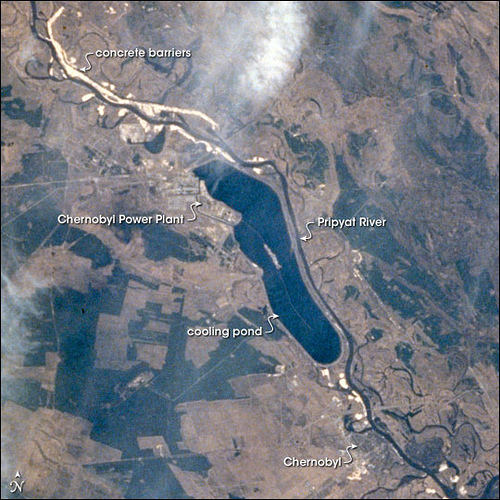
\includegraphics[width=0.5\linewidth]{chernobyl_plant_map}
	\caption{Chernobyl - Map of the plant and colling ponds. The Chernobyl plant and cooling pond are shown in this overhead satellite image captured 10 years after the initial accident}
	\label{fig:chernobylplantmap}
\end{figure}



{\begin{figure}
		\centering
		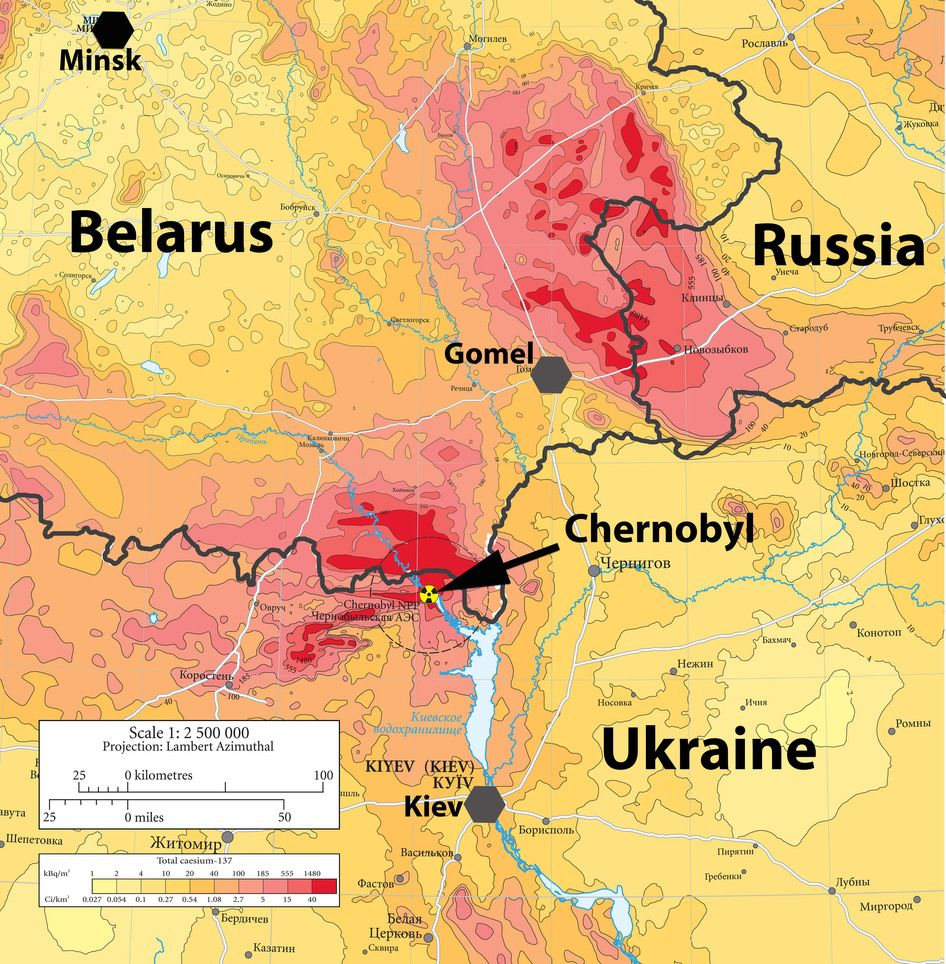
\includegraphics[width=0.5\linewidth]{chernobyl_caesium_137}
		\caption{Chernobyl - Map of caesium-137. The highly radioactive isotope caesium-137 has a medium-term lifespan, with a half-life of around 30 years. However, the damage it causes environmentally is magnified by the ease at which is spreads in the environment due to its water solubility}
		\label{fig:chernobylcaesium137}
	\end{figure}
}{}
\begin{figure}
	\centering
	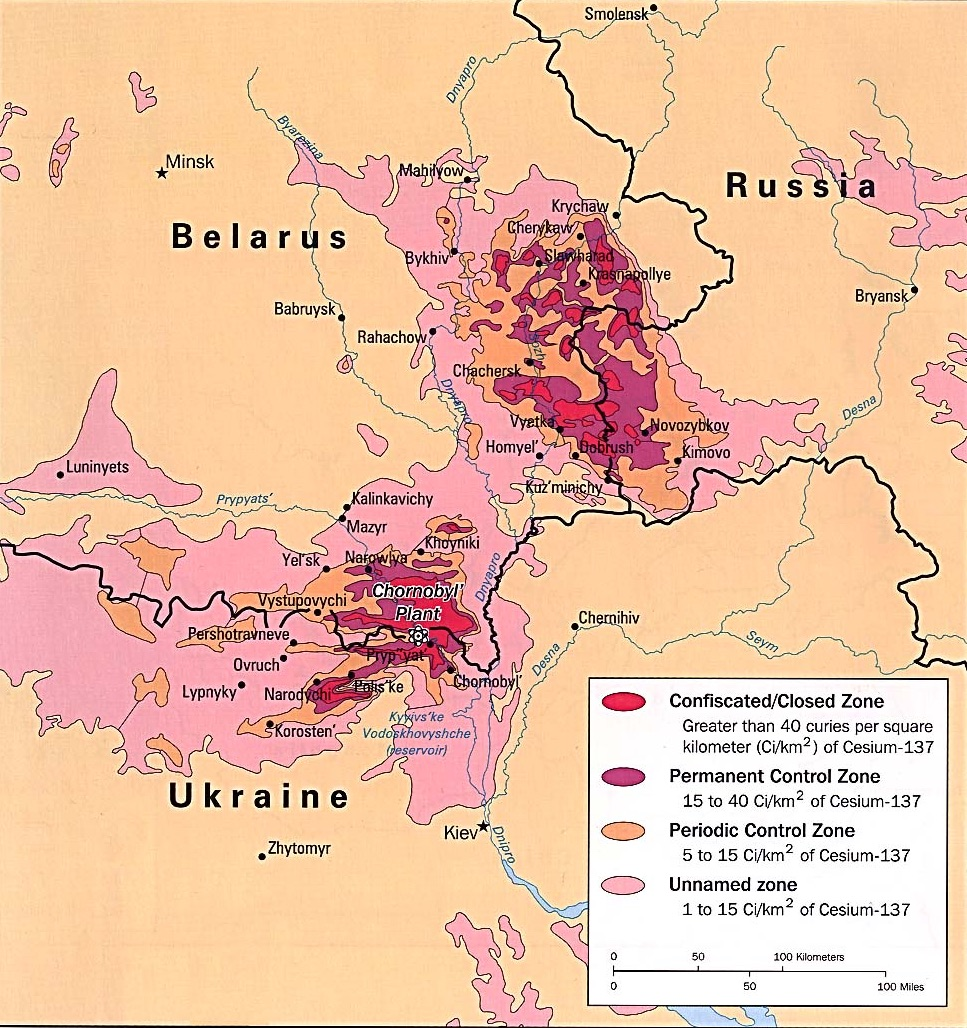
\includegraphics[width=0.5\linewidth]{chernobyl_restricted_zones}
	\caption{Chernobyl - Map of restricted zones - Due to contamination there were exclusion zones set up around the Chernobyl plant over substantial tracts of land in the Ukraine, into Belarus, and affecting as far away as Russia}
	\label{fig:chernobylrestrictedzones}
\end{figure}

\begin{figure}
	\centering
	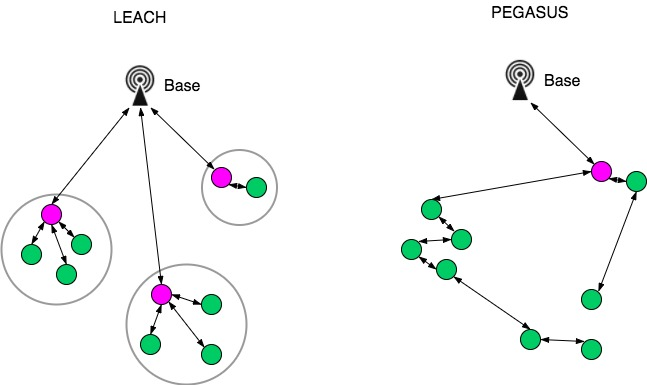
\includegraphics[width=0.7\linewidth]{WSN_simulation_standard_algorithms}
	\caption{WSN standard algorithms - Some standard algorithms for networking in WSN. LEACH uses cluster of nodes each with a lead node for data aggregation and coordination which is rotated periodically to balance power usage. PEGASUS uses chains of nodes with one lead node communicating to the base station.}
	\label{fig:wsnsimulationstandardalgorithms}
\end{figure}

In the event of an incident at a nuclear facility there is a risk that there can be leaks of contaminated radioactive material. This can occur as an atmospheric release or as water that has passed through the cooling system escapes directly into the ground water around the facility instead of being captured in storage ponds for decontamination. In the case of a serious meltdown event such as Chernobyl \cite{Steinhauser2014, Evangeliou2016, Konoplev1992, Fesenko2007, Kortov2013} shown in Figure \ref{fig:chernobylplantmap} we can see a large release of radioactive material into the atmosphere which is then spread globally by winds, contaminating large swathes of the local geographical area, europe, and beyond. We also see this in the many events doumented at the troubled Indian Point plant\cite{TheGuardian} and others where atmospheric releases and ground water contimation have happened repeatedly to varying scales over many years.                                                                                                                                                                                                                                                                                                                                                                                                                                                                                
\newline
\newline


In Chernobyl, lethal levels of radiation were spread over large expanses of remote terrain and have persisted for decades, the land remaining sealed off and uninhabited for over 30 years. These levels mean that humans cannot spend significant time inside the contamination zone without risking rapidly succumbing to the effects of radiation poisoning. Figures \ref{fig:chernobylcaesium137} and \ref{fig:chernobylrestrictedzones} show the contamination areas resulting from the release of the radioactive isotope caesium-137 and corresponding human exclusion zones. Situations like this are unfortunately not that uncommon, although not frequently at such a devastating scale as the Chernobyl or Fukishima disasters. The environmental degradation, essential monitoring characteristics, and harsh external conditions for both humans and machines shown in these cases will prove a fitting and practical testbed for a sensor network deployment based around our agent system.
\newline
\newline


Wide area radioactive contamination gives us a real-world condition that draws out the reasons behind some of the assumptions and criteria used to drive the agent systems learning and operation. In particular, there can be little to no human involvement in deployment or maintenance of sensors deployed to such an environment, the risk to life is simply too large. With this in mind, deployment of sensors is likely to be at-a-distance, and in being so, will have relatively ad-hoc placement. For example, sensors dropped from \textit{Unmanned Aerial Vehicles (UAV)} with no ability to place or move the sensors once released. With a contamination event we may also require sensor readings for many decades, how the adaptation and resilience of an agent-based sensor depoyment can provide for that would prove extremely beneficial to its viability as a solution. Lastly we will see how we can utilise the learning-guided inter-agent linking of the system to give us a robust and resilient networking capability. In addition, dependent on our strategy we can target optimisation of energy utilisation for these low-power remote sensor systems, or should more accurate data be required we can adapt to preferring a greater amount of more granular aggregation of data but at a higher energy cost. 




\subsection{Networking and routing in E-WSN}

In real world deployments it has shown to have been key to balance network robusiness and resilience to damage, alongside the demanding nature of the low energy usage requirements, in order to make the deployments practical, maintainable, and cost-effective. Aside from standard star and peer-to-peer network topologies \cite{Oliveira2011} there have been efforts to develop more targeted architectures based on experience of past WSN \ref{Singh2017, BaniHani, Mahapatra2015, MdZin2014}. Figure \ref{fig:wsnsimulationstandardalgorithms} shows two such algorithms illustrating generalised groupings of these approaches. LEACH uses the idea of sub-clusters of nodes with a nominated lead node that acts as the co-ordintaor and broadcaster of the data back to a base station. These lead nodes are on-hop in that they broadcast directly to the base station, the energy drain caused by this is mitigated by occasionally rotating the lead nodes within the cluster. PEGASUS shows the other main approach to networking with one node acting as the lead node to orchestrate communication with the base station, but there is a multi-hop chain of sub-nodes that relay data through the system using a nearest-neighbour strategy for data request and return. Should a node in the chain go down then the chain will align itself to reform a complete chain back to the base station again. 
\newline
\newline


Comparing these standard algorithms back to the agent system we can see both the similarities with both approaches, but also substantial benefits of the agent-based learning enhancements. The hierarchical approach to agent networking is similar to that we take here, and has been investigated for holoarchy-style agent learning systems such as that of Holmesparker et al \ref{Holmesparker}. The agent system we have set out has both clusters and chains of nodes and clusters as a natural outcome of its operation, with both single-hop and multi-hop both possible outcomes of the structure development through learning links and channels. The networking behaviour is shaped by the definition of local neighbourhood learning for agents and is guided by the higher-level information conveyed by rewards rather than any explicit definitions of networking or agent-system design patterns. While a hierarchical design with lead-agents learning to guide teams of other agents may bear some resemblance to our neighbourhood learning based system, in practice the behaviours within our system are flexible and self-organised to a much greater extent. Scalability itself is incorporated automatically as a direct outcome of placing constraints on neighbourhood formations.
\newline
\newline
\begin{figure}
	\centering
	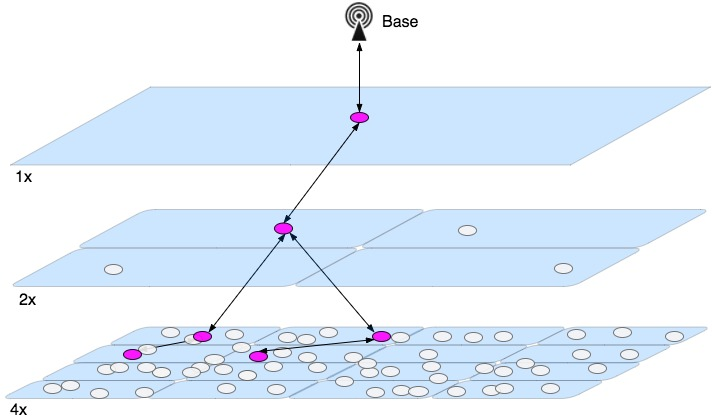
\includegraphics[width=0.7\linewidth]{WSN_hierarchical_resolution}
	\caption{Agent system hierarchical neighbourhood resolution - This diagram shows one of the possible modes of hierarchical networking that can be formed by the agent system through per-agent local neighbourhood learning. The initial agent passes requests through smaller and smaller neighbourhoods until the granulaity of the data meets that of the request}
	\label{fig:wsnhierarchicalresolution}
\end{figure}
\begin{figure}
	\centering
	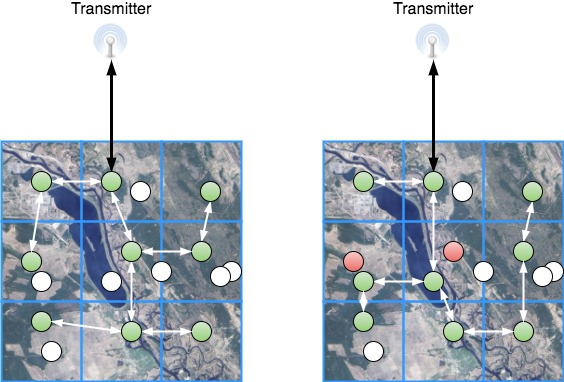
\includegraphics[width=0.7\linewidth]{WSN_simulation_map_failure_adaptation}
	\caption{WSN simulation failure adaptation - The first figure shows a set of agents aggregating data across a defined granularity geographical area using their learned neighbourhoods. In the second we see the adaptation of each agents local neighbourhood as they individually react to device failures}
	\label{fig:wsnsimulationmapfailureadaptation}
\end{figure}

The idea of nearest-neighbour is also applied, but in a more flexible manner and at a higher-level abstraction. While there are definite physical and geographical consequences of deployment such as the range of the transceiver and occlusion behind objects, the agents learn routes with a much wider range of information. Elements such as transfer rate and reliability are large factors in the shape of the reward signals received by agents, but the signal for local neighbourhood formation contains a multitude of other factors and can also be shaped to fit the desired application. So congestion, data consistency, energy cost for transmission and many other factors could be used as elements of the reward heuristic, giving the agents local neighbourhood the shape that best meets with our particular demands on a situational basis. Figure \ref{fig:wsnhierarchicalresolution} illustrates how the agent system works with hierarchical clusters of local neighbourhoods. In reality, the diagram masks the dynamic nature of these neighbourhoods for each agent. Additionally the route through the network of any requests is heavily dependent on the agent that receives an initial request as its neighbourhood will heavily influence the subsequent paths of the requests.
\newline
\newline
With our approach of neighbourhood learning and adaptation for agents we automatically get networking recovery in the event of device failure. Figure \ref{fig:wsn_simulation_failure_adaptation} shows a simplified version of how this might apply when used in agent devices spread over a geographical data, with the grid representing the necessary granularity of the sensor readings. In the first figure, we have an agent aggregating other agent sensor readings as defined by its learned local neighbourhood. We then lose two of the sensors that were on devices that formed the most-optimal data reading request channels in other agents neighbourhoods. The second figure shows how the agents then quickly learn to prioritise data requests over other channels to form an adapted neighbourhood, although this step could also have introduced new channels as part of a state-action space adaptation by the agent to recover connectivity. This shows how we can deploy an agent-system that can adaptively recover from significant outages across the sensor network.


\subsection{Power consumption and recovery}

Another important aspect in the envisaged E-WSN system is the price of inter-agent communication as dictated by the energy consumption of each sensors transceiver while broadcasting. To make the deployment feasible we need a low-energy use system, while still having agents dynamically self-coordintate and using their communication channels to retrieve data readings. With the concept of channels already included within our agent system we can add this easily to the simulation by providing an energy cost to links through these channels. This equates to the power necessary to broadcast throught this communication channel, simulating distance between agents, occlusions, and atmospheric effects that may force higher power requirements on the transeiver if utilised in a real environment. In this way, each message passed through a link will not only shape the subsequent reward through return time, but also through the energy cost of the message. This will ensure that we are not only having agents learn the most efficent data transfer behaviours, but also have the energy efficiency of their requests impact the learning. We also must take in to account the need to spread power distribution across the system. There cannot be a small subset of nodes that are handling the majority of the functionality and therefore the energy usage as their batteries and solar top-up systems will become overwhelmed. Instead we must learn to spread the load, indeed this is exactly what the congestion simulation proviously did through delaying data return times.
\newline
\newline
Now having extended this concept and added an energy consumption measure to agents channels which are proportional to the energy use generated by messages passing through their links, we can use this to accumulate energy consumption rates for those linked-to agents, and use this to drive the requesting agent learning towards adaptation in the face of overloading links. Using $E\textsubscript{cost} $ as the energy cost of making a broadcast request through a link, and $E\textsubscript{rec}$ as the energy recovered by the solar panels of the device per unit of time. We can then use the set of actions on a link $l$ at time $t$ as  $\mathbb{A}_l^t$ to define the actions that cause the link to broadcast, and therefore use energy. We can therefore specify the current energy usage $E\textsubscript{usage} $ of the link as,

\begin{equation}
	E\textsubscript{usage} =  \sum\limits_{i=0}^{t}
	(E\textsubscript{cost} - E_{rec}^{(t-i)})
	\times \mathbb{A}_l^i
\end{equation}
\newline
\newline

We then use the energy usage of a link as a negative factor in our rewards for the requesting agent. Energy costs such as altering links and channels are already encapsulated within the agent system as fixed negative rewards.
	\section{Balancing energy and measurement in a WSN system}
\label{section:problem}
%%%%%%%%%%%%%%%%%% NOTATION %%%%%%%%%%%%%%%%%%%%%%%%%%
\newcommand{\varTime}[2]{\phi}
\newcommand{\setTime}[2]{\Phi}
\newcommand{\varAtomicTask}[2]{\varSymbol{at}{#1}{#2}}
\newcommand{\setAtomicTask}[2]{\setSymbol{AT}{#1}{#2}}
\newcommand{\varCompositeTask}[2]{\varSymbol{ct}{#1}{#2}}
\newcommand{\setCompositeTask}[2]{\setSymbol{CT}{#1}{#2}}

\newcommand{\varAgent}[2]{g_{#1}^{#2}}
\newcommand{\setAgents}[2]{G_{#1}^{#2}}

\newcommand{\powerSetAgents}[2]{\powerSetSymbol{G_{#1}^{#2}}{}{}}
\newcommand{\varIdleAgent}[2]{\varAgent{i}{}}  
\newcommand{\varSleepAgent}[2]{\varAgent{s}{}}  
\newcommand{\varChildAgent}[2]{\varAgent{c}{}}    
\newcommand{\varParentAgent}[2]{\varAgent{p}{}}

\newcommand{\varOrchestrationEnergy}[2]{e_{orch}}
\newcommand{\varTransmissionEnergy}[2]{e_{trans}}
\newcommand{\varReceiverEnergy}[2]{e_{recv}}
\newcommand{\varSensorEnergy}[2]{e_{sens}}
\newcommand{\varIdleEnergy}[2]{e_{idle}}
\newcommand{\functionTaskRange}[2]{
	\functionSignature{\mathit{range}}
	{\varAtomicTask{}{}}
}


\newcommand{\functionAtomicTaskEnergyConsumptionSignature}[2]{
	\functionSignature{atec}{\varAtomicTask{}{}}}

\newcommand{\formalAtomicTaskEnergyConsumption}[2]{
	\functionFormal{atec}
	{\setAtomicTask{}{}}
	{\setRealNumbersNonNegative{}{}}}
%%%%%%%%%%%%%%%%%%%%%%%
\newcommand{\symbolDataAcquisition}[2]{\setSymbol{DAQ}{#1}{#2}}
\newcommand{\symbolTransmission}[2]{\setSymbol{TX}{#1}{#2}}
\newcommand{\symbolReceiver}[2]{\setSymbol{RX}{#1}{#2}}
\newcommand{\symbolWakeUpRadio}[2]{\setSymbol{WUR}{#1}{#2}}


\newcommand{\functionSystemEnergyDistribution}[2]{
	\functionSignature{sed_{\varTime{}{}}}
	{\setAgent{}{}}
}
\newcommand{\functionSystemEnergyVariability}[2]{
	\functionSignature{sev_{\varTime{}{}}}
	{\setAgents{}{}}
}
\newcommand{\functionAgentEnergyTotal}[2]{
	\functionSignature{aet_{\varTime{}{}}}
	{\varAgent{#1}{#2}}
}

\newcommand{\functionProbabilityInit}[2]{
	\functionSignature{pinit}{\varAgent{}{}}
}
\newcommand{\functionProbabilityRand}[2]{
	\functionSignature{prand}{\varAgent{}{}}
}
\newcommand{\functionProbabilityWear}[2]{
	\functionSignature{pwear}{\varAgent{}{}}
}
\newcommand{\functionProbabilityFail}[2]{
	\functionSignature{pfail}{\varAgent{}{}}
}
\newcommand{\varConstantInit}[2]{{C}{INIT}^{#2}}
\newcommand{\varConstantRand}[2]{{C}{RAND}^{#2}}
\newcommand{\varConstantWear}[2]{{C}{WEAR}^{#2}}
\newcommand{\varEnergyInit}[2]{{E}{INIT}^{#2}}
\newcommand{\varEnergyWear}[2]{{E}{WEAR}^{#2}}

%%%%%%%%%%%%%%%%%% NOTATION %%%%%%%%%%%%%%%%%%%%%%%%%%
\newcommand{\varSample}[2]{\varSymbol{\psi}{#1}{#2}}
\newcommand{\setSample}[2]{\setSymbol{\Psi}{#1}{#2}}
\newcommand{\varMeasurement}[2]{\varSymbol{m}{#1}{#2}}
\newcommand{\varPeriod}[2]{\varSymbol{p}{#1}{#2}}
\newcommand{\varError}[2]{\varSymbol{\omega}{#1}{#2}}
\newcommand{\setError}[2]{\setSymbol{\Omega}{#1}{#2}}
\newcommand{\tupleVarSample}[2]{
	(\varTime{#1}{#2}, \varMeasurement{#1}{#2}, \varError{#1}{#2})
}
\newcommand{\tupleSetSample}[2]{
	(\setTime{#1}{#2}, \setMeasurement{#1}{#2}, \setError{#1}{#2})
}

%%%%%%%%%%%%%%%%%% NOTATION %%%%%%%%%%%%%%%%%%%%%%%%%%
\newcommand{\varBatteryEnergy}[2]{\varSymbol{e}{\varAgent{}{}}{#2}}
\newcommand{\setBatteryEnergy}[2]{\setSymbol{E}{#1}{#2}}
\newcommand{\varBatteryEnergyMax}[2]{\varBatteryEnergy{\varAgent{}{}}{max}}

%%%%%%%%%%%%%%%%%%%%%%%%%%%%%%%%%%%%%%
\newcommand{\varLocation}[2]{\varSymbol{loc}{#1}{#2}}
\newcommand{\setLocation}[2]{\setSymbol{LOC}{#1}{#2}}
\newcommand{\formalVarLocation}[2]{(x,y)}
\newcommand{\formalSetLocation}[2]{(\setRealNumbers{}{} \times \setRealNumbers{}{})}

\newcommand{\functionDeployment}[2]{
	\ifx \\1\\
	\functionSignature{conf}{\setAgents{}{}}
	\else
	\functionSignature{conf}{#1}
	\fi 
}
\newcommand{\formalDeployment}[2]{\functionFormal{conf}{\setAgents{}{}}{(\setRealNumbersNonNegative{}{} \times \setRealNumbersNonNegative{}{})}}
\newcommand{\functionTaskArc}[2]{\functionSignature{path}{\varAtomicTask{}{}}}
\newcommand{\formalTaskArc}[2]{\functionFormal{path}{\setAtomicTask{}{}}{\powerSetAgents{}{}}}
\newcommand{\functionTaskDemandPoint}[2]{\functionSignature{dp}{\varAtomicTask{}{}}}
\newcommand{\formalTaskDemandPoint}[2]{\functionFormal{dp}{\setAtomicTask{}{}}{(\setRealNumbersNonNegative{}{} \times \setRealNumbersNonNegative{}{})}}
\newcommand{\varActiveAgent}[2]{\varAgent{#1}{\oplus}}
\newcommand{\varInactiveAgent}[2]{\varAgent{#1}{\ominus}}
\newcommand{\varSensingAgent}[2]{\varAgent{#1}{\ast}}
\newcommand{\varSinkAgent}[2]{\varAgent{#1}{\Delta}}

\newcommand{\varEnergy}[2]{\varSymbol{e}{#1}{#2}}
\newcommand{\setEnergy}[2]{\setSymbol{E}{#1}{#2}}
%%%%%%%%%%%%%%%%%%%%%%%%%%%%%%%%%%%%%
\newcommand{\varResource}[2]{\varSymbol{r}{#1}{#2}}
\newcommand{\setResource}[2]{\setSymbol{R}{#1}{#2}}
\newcommand{\formalTaskResourceAllocation}[2]{
	\functionFormal{ra}
	{\setAgents{}{} \times \setAtomicTask{}{}}
	{\powerSetSymbol{\setResource{}{} \times \setRealNumbersNonNegative{}{}}{}{}}
}
\newcommand{\functionTaskResourceAllocation}[2]{
	\functionSignature{ra}
	{\varAgent{}{}, \varAtomicTask{}{}}
}
%%%%%%%%%%%%%%%%%%%%%%%%%%%%%%%%%%%%%%%%
	%%%%%%%%%%%%%%%%%%%%%%%%%%%%%%%%%%%%%%
\newcommand{\varLocation}[2]{\varSymbol{loc}{#1}{#2}}
\newcommand{\setLocation}[2]{\setSymbol{LOC}{#1}{#2}}
\newcommand{\formalVarLocation}[2]{(x,y)}
\newcommand{\formalSetLocation}[2]{(\setRealNumbers{}{} \times \setRealNumbers{}{})}

\newcommand{\functionDeployment}[2]{
\ifx \\1\\
\functionSignature{conf}{\setAgents{}{}}
\else
\functionSignature{conf}{#1}
\fi 
}
\newcommand{\formalDeployment}[2]{\functionFormal{conf}{\setAgents{}{}}{(\setRealNumbers{}{} \times \setRealNumbers{}{})}}
\newcommand{\functionTaskArc}[2]{\functionSignature{arc}{\varAtomicTask{}{}}}
\newcommand{\formalTaskArc}[2]{\functionFormal{arc}{\setAtomicTask{}{}}{\powerSetAgents{}{}}}
\newcommand{\functionTaskDemandPoint}[2]{\functionSignature{dp}{\varAtomicTask{}{}}}
\newcommand{\formalTaskDemandPoint}[2]{\functionFormal{dp}{\setAtomicTask{}{}}{(\setRealNumbersNonNegative{}{} \times \setRealNumbersNonNegative)}}
\newcommand{\varActiveAgent}[2]{\varAgent{#1}{\oplus}}
\newcommand{\varInactiveAgent}[2]{\varAgent{#1}{\ominus}}
\newcommand{\varSensingAgent}[2]{\varAgent{#1}{\ast}}
\newcommand{\varSinkAgent}[2]{\varAgent{#1}{\Delta}}

\newcommand{\varEnergy}[2]{\varSymbol{e}{#1}{#2}}
\newcommand{\setEnergy}[2]{\setSymbol{E}{#1}{#2}}
%%%%%%%%%%%%%%%%%%%%%%%%%%%%%%%%%%%%

%%%%%%%%%%%%%%%%%%%%%%%%%%%%%%%%%%%%%%

\todo[inline]{PROBLEM - SYSTEM}

\begin{figure}
\centering 
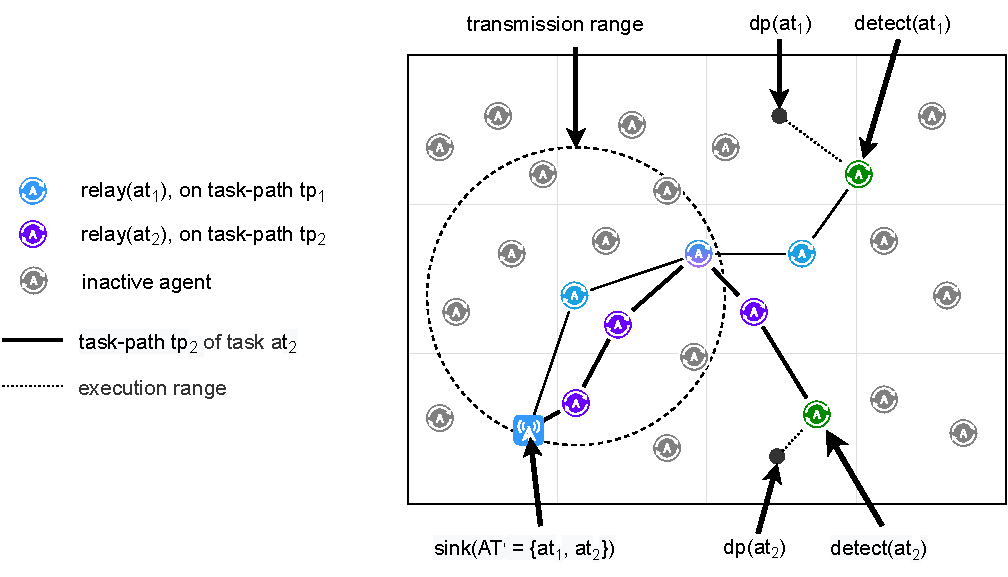
\includegraphics[width=0.9\linewidth]{grid_concept}
\caption[WSN deployment terminology]{WSN deployment terminology}
\label{fig:gridconcept}
\end{figure}

\subsubsection*{Deployment configuration}
Given a geographical area to monitor, we can overlay a two dimensional grid of real numbers, allowing us to associate a deployed set of nodes, or agents, $\setAgents{}{}$, with a corresponding location, $\formalVarLocation{}{} \in \formalSetLocation{}{}$. on the grid. This describes the \textit{deployment configuration} of those agents, a mapping from agents to real valued tuples representing their location,  $\formalDeployment{}{}$.


\begin{definition}[Composite task]
	A \textit{composite task}, is composed of $N$ atomic tasks $\varCompositeTask{}{} = \lbrace \varAtomicTask{i}{} \rbrace_{i=0}^N$ where for each of the $i\in N$ grid blocks of the systems geographical grid area.
\end{definition}

\begin{definition}[Atomic task]
	An \textit{atomic task} $\varAtomicTask{\varLocation{}{}}{}$ is a task to take a measurement at a target location $\varLocation{}{}$. The task can be completed by any agent, no matter its distance from the target point.
\end{definition}

\newcommand{\functionTaskResourceAllocation}[2]{
	\functionSignature{ra_{\varAgent{}{}}}
	{\varAtomicTask{}{}}
}
\begin{definition}[Task resource allocation]
	XXX
\end{definition}


\begin{definition}[Demand point]
	A \textit{demand point} is a specific location associated with an atomic task $\functionTaskDemandPoint{}{}$.
\end{definition}


\subsubsection*{Node roles and task arcs}
%%%%%%%%%%%%%%%%%%%%%%%%%%%%%%%%%%%%%%%%%%%%
\newcommand{\formalSinkRole}[2]{
	\functionFormal{sink}
	{\setAtomicTask{}{} \times \setAgents{}{}}
	{\powerSetAgents{}{}}
}
\newcommand{\formalSenseRole}[2]{
	\functionFormal{sense}
	{\setAtomicTask{}{} \times \setAgents{}{}}
	{\powerSetAgents{}{}}
}
\newcommand{\formalActiveRole}[2]{
	\functionFormal{active}
	{\setAtomicTask{}{} \times \setAgents{}{}}
	{\powerSetAgents{}{}}
}
\newcommand{\formalIdleRole}[2]{
	\functionFormal{idle_{\setTime{}{}}}
	{\setAgents{}{}}
	{\setAgents{}{}}
}
\newcommand{\formalSleepRole}[2]{
	\functionFormal{sink_{\setTime{}{}}}
	{\setAgents{}{}}
	{\setAgents{}{}}
}
\newcommand{\functionSinkRole}[2]{\functionSignature{sink}{\varAtomicTask{}{}, \setAgents{}{}}}
	
\newcommand{\functionSenseRole}[2]{\functionSignature{sense}{\varAtomicTask{}{}, \setAgents{}{}}}
\newcommand{\functionActiveRole}[2]{\functionSignature{active}{\varAtomicTask{}{}, \setAgents{}{}}}
\newcommand{\functionIdleRole}[2]{\functionSignature{idle}{\varAtomicTask{}{}, \setAgents{}{}}}
\newcommand{\functionSleepRole}[2]{\functionSignature{sleep}{\varAtomicTask{}{}, \setAgents{}{}}}


We can distinguish agents by the role they play in a given atomic task.
\begin{itemize}
	\item A \textit{sink node} of an atomic task $\varAtomicTask{}{}$ is the agent that first receives the corresponding composite task, and will broadcast the results, $\formalSinkRole{}{}$.
	\item A \textit{sensing node} is the agent that executes the atomic task and so performs the sensor measurement, $\formalSenseRole{}{}$.
	\item An \textit{active node} is an agent that participates in sub-allocating, or routing, that task, but is neither a sink agent nor a sensing agent, $\formalActiveRole{}{}$..
	\item An \textit{idle node} does not participate in the specific task, but is for other tasks during a time period $\setTime{}{}$, $\formalIdleRole{}{}$.
	\item An \textit{sleeping node} does not participate in any of the tasks in the system during a time period $\setTime{}{}$, $\formalSleepRole{}{}$.
\end{itemize}

With these roles in mind, we can now define the \textit{task arc}

\begin{definition}[Atomic task arc]
	A \textit{atomic task arc} is a mapping of atomic tasks to ordered sequence of agents $\formalTaskArc{}{}$ that each atomic task $\varAtomicTask{}{}$ is sub-allocated to. The first agent is the agent that has received the initial composite task, and the last agent is the agent that executes the atomic task such that, 
	$\functionTaskArc{}{} = \lbrace \varSinkAgent{}{}, \varActiveAgent{i}{}, \varSensingAgent{}{} \rbrace_{i=1}^{n}$. Where there are $n$ active agents sub-allocating the task between the sink and sensing agents.
\end{definition}


	\subsection{Energy consumption and availability}
\label{section:energy_consumption}

We quantify an \textit{atomic task energy consumption}, $\formalAtomicTaskEnergyConsumption{}{}$, as the energy used by a task paths' nodes in executing the atomic task \footnote{See definition of key requirements, \ref{requirement:energy}, in Section \ref{section:background}}. This is composed of,
 \begin{itemize}
 	\item \textit{Transmission energy}, $\varTransmissionEnergy{}{}$, the energy used by nodes to  send a message, such as when allocating a task to another node or returning a task result. 
 	\item \textit{Receiver energy}, $\varReceiverEnergy{}{}$, the energy used by a node to receive a message. 
 	 \item \textit{Sensor energy}, $\varSensorEnergy{}{}$,the energy used by a node to execute an atomic measurement task.
 \end{itemize}
For simplification, we assume that these values are constants in a given system. For a given task-path, the combined energy usage will be,
\begin{align}
\functionAtomicTaskEnergyConsumptionSignature{}{} 
&= 
\underbrace{(\varTransmissionEnergy{}{} + \varReceiverEnergy{}{})}_{\text{sink node}}
+ \underbrace{
	2 (\varTransmissionEnergy{}{} + \varReceiverEnergy{}{})
 	(\funcSize{(\functionTaskArc{}{}}{} -2)
}_{\text{active nodes}}
+ \underbrace{
	 (
	 	\varTransmissionEnergy{}{}
	 	+ \varReceiverEnergy{}{}
	 	+ \varSensorEnergy{}{}
	 )
 }_{\text{sensor node}}  
\end{align}
Although nodes would still use energy when in an idle power saving mode, or sleep mode, we disregard these for this formulation as we look to optimise the active node power usage only. There are other algorithms that can be used to optimise the cycling of power cell usage \citep{Escolar2014}.

%%%%%%%%%%%%%%%%%%%%%%%%%%%%%%%%%%%%%%%%%
\newcommand{\formalAgentEnergyAvailable}[2]{
	\functionFormal{\mathit{fe}}
	{\setAgents{}{}}
	{\setRealNumbersUnit{}{}}
}
\newcommand{\functionAgentEnergyAvailable}[2]{
	\functionSignature{\mathit{fe}_{\varTime{}{}}}
	{\varAgent{}{}}
}
\newcommand{\functionEnergyVariability}[2]{
	\ifx \\#1\\
	\functionSignature{rev_{\varTime{}{}}}
	{\setAgents{}{}}
	\else
	\functionSignature{rev_{\varTime{}{}}}{#1}
	\fi
}

\newcommand{\functionEnergyAvailable}[2]{
	\ifx \\#1\\
	\functionSignature{ea_{\varTime{}{}}}{\setAgents{}{}}
	\else
	\functionSignature{ea_{\varTime{}{}}}{#1}
	\fi
}
The \textit{fractional agent energy} maps an agent to its available energy, as a fraction of its energy sources maximum capacity, $\formalAgentEnergyAvailable{}{}$. We can then specify the \textit{fractional energy availability}, as the sum-average of the agent energy of all agents in a set $\setAgents{}{}$.
\begin{equation}
	\functionEnergyAvailable{}{} 
	= \dfrac{\sum_{\forall \varAgent{}{} \in \setAgents{}{}} \functionAgentEnergyAvailable{\varAgent{i}{}}{}}
	{\funcSize{\setAgents{}{}}}
\end{equation}
To optimise for distribution of energy usage we minimise the variance\footnote{Using the standard definition of variability of a discrete set $X$, $\sigma^2(X) = \frac{\sum (x_i - \bar{x})^2}{\funcSize{X}-1}$} of the fractional agent energy values. As we look to optimise by maximising across multiple goals, and the values of $\functionAgentEnergyAvailable{}{}$ are bounded by $[0, 1]$, we can rephrase this as maximising the distance between the variance and the maximum possible, $1/4$. So we use the \textit{relative energy variability} as our distribution measurement,
\begin{equation}     	
	\functionEnergyVariability{}{} 
	= \frac{1}{4} - \sigma^2(
	\lbrace \functionAgentEnergyAvailable{}{}
	\rbrace_{\forall \varAgent{}{} \in \setAgents{}{}}
	)
\end{equation}



	%%%%%%%%%%%%%%%%%%%%%%%%%%%%%%%%%%%%%%%%%%
\newcommand{\formalAgentEnergyAvailable}[2]{
	\functionFormal{fae}
	{\setAgents{}{}}
	{\setRealNumbersUnit{}{}}
}
\newcommand{\functionAgentEnergyAvailable}[2]{
	\functionSignature{fae_{\varTime{}{}}}
	{\varAgent{}{}}
}


\subsection{Energy in the system}
\newcommand{\functionEnergyVariability}[2]{
\ifx \\#1\\
	\functionSignature{ev_{\varTime{}{}}}
	{\setAgents{}{}}
\else
	\functionSignature{ev_{\varTime{}{}}}{#1}
\fi
}
\newcommand{\functionEnergyAvailable}[2]{
\ifx \\#1\\
	\functionSignature{ea_{\varTime{}{}}}{\setAgents{}{}}
\else
	\functionSignature{ea_{\varTime{}{}}}{#1}
\fi
}
\todo[inline]{PROBLEM - ENERGY}
\subsubsection{Availability of energy}

The \textit{fractional agent energy} maps the an agent to its available energy, as a fraction of the batteries' maximum capacity, $\formalAgentEnergyAvailable{}{}$. We can then specify the \textit{energy availability}, as the sum of the fractional agent energy of all agents in a set $\setAgents{}{}$.
	\begin{equation}
		\functionEnergyAvailable{}{} 
		= \sum_{\forall \varAgent{}{} \in \setAgents{}{}} \functionAgentEnergyAvailable{\varAgent{i}{}}{}
	\end{equation}
and the \textit{energy variability} as the variance\footnote{Using the standard definition of variability of a discrete set $X$, $\sigma^2(X) = \frac{\sum (x_i - \bar{x})^2}{\funcSize{X}-1}$} of energy available to those agents.
	\begin{equation}     	
		\functionEnergyVariability{}{} 
		= \sigma^2(
			\lbrace \functionAgentEnergyAvailable{}{}
			\rbrace_{\forall \varAgent{}{} \in \setAgents{}{}}
		)
	\end{equation}

\newcommand{\functionTaskEnergyConsumption}[2]{
	\functionSignature{tec}
	{\varAtomicTask{}{}}
}
\todo[inline]{Define task consumption in terms of arc}
The \textit{task energy consumption} is the energy used by all agents in the system in executing an atomic task $\varAtomicTask{}{}$. Transmission energy, $\varTransmissionEnergy{}{}$, the power used by a node to  broadcast a message to allocate a task to another node, or reply with a task result. Receiver energy is the energy used by an agent to receives a message. Both transmission and receiving in an atomic task sequence of allocations involve all members of the arc twice, apart from the sink and sensing nodes which will only transmit and receive once. Note, we make the assumption that the energy of a broadcast of receipt of a message is independent of range. 
\begin{equation}
	\functionTaskEnergyConsumption{}{} 
	= 2\varTransmissionEnergy{}{} (\funcSize{\functionTaskArc{}{}}{} - 1)
	+ 2\varReceiverEnergy{}{} (2 \funcSize{\functionTaskArc{}{}}{} - 1)
\end{equation}
Although nodes would still use energy when in an idle power saving mode, or sleep mode, we disregard these for this formulation as we look to optimise the active node power usage only. There are other algorithms that can be used to optimise the cycling of power cell usage \cite{DUMMY}.
\subsubsection{Energy consumption}
\newcommand{\functionSystemEnergyConsumption}[2]{
	\functionSignature{sec}
	{\setCompositeTask{}{}}
}
\todo[inline]{Include orchestration energy?}
We can then go on to define the \textit{system energy consumption} as the energy used by all of the composite tasks $\setCompositeTask{}{}$ that are completed within a time period $\setTime{}{}$.
\todo[inline]{This isnt right wrt idle and sleeping, and how it works with tec}
\begin{equation}
	\functionSystemEnergyConsumption{}{} 
	= 
	\sum_{\forall \varCompositeTask{}{} \in \setCompositeTask{}{}}
	\sum_{\forall \varAtomicTask{}{} \in \varCompositeTask{}{}} \functionTaskEnergyConsumption{}{}
	+ \varIdleEnergy{}{} \sum \functionIdleRole{}{}
	+ \varSleepEnergy{}{} \sum \functionSleepRole{}{}
\end{equation}


	%%%%%%%%%%%%%%%%%
\newcommand{\functionAtomicTaskQualitySignature}[2]{
	\functionSignature{q_{\varAgent{}{}, \varTime{}{}}} {\varAtomicTask{}{}}
}
\newcommand{\functionCompositeTaskValue}[2]{
	\functionSignature{ctv}{\varCompositeTask{}{}}
}
%%%%%%%%%%%%%%%%%%%%%%%%%%%%%%%%%%%%%%%%%%%%
\subsubsection*{Quality of measurement}

\todo[inline]{PROBLEM - TASKS}

A sensor is capable of taking a measurement of the radiation levels at the location of its sensor, which may be a distance away from the tasks' demand point. In addition, the longer the sample time the more energy is used, but the more accurate the reading will be \cite{dummy}. We therefore define the value of the measurement as follows,

\begin{definition}[Atomic task quality]
	The \textit{atomic task quality} of an atomic task $\varAtomicTask{}{}$ is a function of the distance of the task from the requested position, and the amount of energy used to make the measurement.
	\begin{equation}
		\functionAtomicTaskQualitySignature{}{} = \functionTaskResourceAllocation{}{} \times \funcSize{
				\functionTaskDemandPoint{}{} - \functionDeployment{\varAgent{}{}}{}
		}{}
	\end{equation}
\end{definition}

\begin{definition}[Composite task value]
	The \textit{composite task value} of $\varCompositeTask{}{}$ is a measure of the quality of the atomic tasks that compose it, the remaining energy available to the agents that completed those atomic tasks, and the overall variability of the energy over those agents. 
	\begin{equation}
		\functionCompositeTaskValue{}{} = 
		\sum_{\forall \varAtomicTask{}{} \in \varCompositeTask{}{}}
		\big\lbrack
		\alpha\underbrace{\functionEnergyAvailable{\functionTaskArc{}{}}{}}_{\text{energy available}}
		+ \beta\underbrace{\functionEnergyInverseVariability{\functionTaskArc{}{}}{}}_{\text{energy distribution}}
		+ 
		\gamma\underbrace{\functionAtomicTaskQualitySignature{}{}}_{\text{task quality}}
		\big\rbrack
	\end{equation}
Where $\alpha$, $\beta$, and $\gamma$, are XXXX that can be chosen to weight the optimisation more strongly between the different factors.
\end{definition}
By maximising composite task quality we then will increase,
\begin{itemize}
	\item The energy availiable in the system, minimising the overall battery power consumption.
	\item The distribution of energy use across the nodes. To maximise the usable lifetime of nodes, we want to make sure wear is spread across nodes. 
	\item The quality of atomic tasks, the will not only improve the accuracy of readings, but will also invoke a penalty of poor task coverage, as failed tasks have the lowest quality.
\end{itemize}

	The utility of the system can be increased by; improving the quality of task completions, minimising energy consumption, and distributing energy usage more evenly across agents. In doing so, the necessary WSN properties of coverage, resilience and system lifetime \footnote{As discussed in Section \ref{section:background:requirements}.} should also increase. Using the concept of success of an atomic task, we now define how we can measure these within the system.

%%%%%%%%%%%%%%%%%%%%%%%%%%%%%%
\newcommand{\varQualityMin}[2]{c_{\textit{qual}}}

\newcommand{\formalAtomicTaskSuccess}[2]{
	\functionFormal{success}
	{\setAtomicTask{}{}}
	{\setIntegersBinary{}{}}
}
\newcommand{\functionAtomicTaskSuccess}[2]{
	\functionSignature{success}{\varAtomicTask{#1}{#2}}
}

\newcommand{\formalCompositeTaskCoverage}[2]{
	\functionFormal{taskcov}
	{\setCompositeTask{}{}}
	{\setRealNumbersUnit{}{}}
}
\newcommand{\functionCompositeTaskCoverage}[2]{
	\functionSignature{taskcov}{\varCompositeTask{}{}}
}


\newcommand{\functionSystemCoverage}[2]{
	\functionSignature{syscov}{\setAtomicTaskInstance{}{}}
}
%%%%%%%%%%%%%%%%%%%%%%%%%%%%%%%%%%%%%%%%%%

\paragraph{Task success}
\label{section:success}
In real-life scenarios, when the quality of an atomic task completion falls below a certain \textit{quality threshold}, $\varQualityMin{}{}$, the result may no longer be useful or relevant to the system, e.g. when an agent takes a sensor measurement, but so far away from the corresponding tasks' demand point that the result is not useful.  We formalise this concept as the atomic task mapping $\formalAtomicTaskSuccess{}{}$ where;

\begin{equation}
	 \functionAtomicTaskSuccess{}{}
	 = 
	\begin{cases}
		1, & \text{if } \functionAtomicTaskQualitySensor{}{} > \varQualityMin{}{} \\
		0, & \text{otherwise}
	\end{cases}
\end{equation}

\paragraph{Coverage}
\label{section:coverage}
Given a set of completed atomic tasks, $\setAtomicTaskInstance{}{} \subseteq \setAtomicTask{}{}$, then the \textit{system coverage} of these tasks is the fraction of those tasks which were successful;
\begin{equation}
	\label{eq:coverage}
	\functionSystemCoverage{}{}
	=
	\frac{1}{\funcSize{\setAtomicTaskInstance{}{}}}
	\sum\limits_{\forall \varAtomicTask{}{} \in \setAtomicTaskInstance{}{}}
	\functionAtomicTaskSuccess{}{}
\end{equation}

%%%%%%%%%%%%%%%%%%%%%%%%%%
\newcommand{\functionSymbolResilence}[2]{\functionSymbol{resilience}{#1}{#2}}
\newcommand{\functionResilence}[2]{
	\functionSignature{\functionSymbolResilence{#1}{#2}}
	{\setAtomicTaskInstance{}{}, \setAgent{}{'}, \setAgent{}{} }
}
\paragraph{Resilience}
\label{section:resilience}
A systems' agents may become either permanently or temporarily unavailable through events such as component failures, communication problems, or weather disruption. In these circumstances, relaying atomic tasks to agents that can successfully complete can be complex or even impossible.
 The ability to maintain coverage under these circumstances defines a systems' \textit{resilience}. Specifically, if a system completes a set of atomic tasks $\setAtomicTaskInstance{}{}$, with available agents $\setAgent{}{'}$, out of the system agents $\setAgent{}{}$, then the systems \textit{resilience} can be defined as; 
\begin{equation}
	\functionResilence{}{}
	= 
	\frac{
		\functionSystemCoverage{}{}
	}{
		\funcSize{\setAgents{}{'}} / \funcSize{\setAgents{}{}}
	}
\end{equation}
In this way, a system whose coverage remains high as the number of available agents falls has a higher resilience that a system who coverage drops lower under the same circumstances.


%%%%%%%%%%%%%%%%%%%%%%%%%%%%%%%
 \newcommand{\varCoverageMinimum}[2]{\varSymbol{c}{\textit{life}}{}}
 %%%%%%%%%%%%%%%%%%%%%%%%%%%%%%%
 \paragraph{Lifetime}
 \label{section:lifetime}
 Despite a systems resilience, given enough agents becoming permanently unavailable, some atomic tasks will become impossible to complete successfully, and there will be a deterioration of coverage with time. For a specific system, a minimum coverage value $\varCoverageMinimum{}{}$ for some set of atomic tasks $\setAtomicTaskInstance{}{}$ can be chosen below which the system is judged to be no longer useful. The \textit{lifetime} of the system can then be defined as the time until $\functionSystemCoverage{}{} < \varCoverageMinimum{}{}$.
 
 
\example{Success and coverage}{
	An ocean-monitoring system has a deployment area of $1\text{ km}^2$. An agent $\varAgent{}{}$ takes a salinity measurement $1$ metre away from a demand point of a task $\varAtomicTask{1}{}$, and $900$ metres from that of $\varAtomicTask{2}{}$. The result of $\varAtomicTask{1}{}$ is likely to be close to the actual value at the demand points' location, whereas that of $\varAtomicTask{2}{}$ is so far away as to uncorrelated, and not a practically useful measurement to the system. In this case, $\functionAtomicTaskSuccess{1}{} = 1$ and $\functionAtomicTaskSuccess{2}{} = 0$. So, with $\setAtomicTaskInstance{}{} = \lbrace \varAtomicTask{1}{}, \varAtomicTask{2}{} \rbrace$, the system coverage is $\functionSystemCoverage{}{} = \frac{1}{2}(1 + 0) = 0.5$  
}
	\subsection{System utility}
%%%%%%%%%%%%%%%%%%%%%%%%%%%%
\newcommand{\functionSystemUtility}[2]{\functionSignature{u_{\setTime{}{}}}{\setCompositeTask{}{}}}
%%%%%%%%%%%%%%%%%%%%%%%%%%%%%%%%%
\todo[inline]{Simplify this}
Given the system goal is balanced between the multiple objectives of, minimising the overall energy used by composite tasks, the energy variance between system agents, while maximising the quality of composite tasks, and the composite task coverage, then the utility of the system is,

\begin{definition}[System utility]
	The \textit{system utility} over a time period $\setTime{}{}$ is the sum of the values of all the composite tasks $\setCompositeTask{}{}$ completed during that period.
	\begin{equation}
		\functionSystemUtility{}{} = \sum_{\forall \varCompositeTask{}{} \in \setCompositeTask{}{}}
		\functionCompositeTaskQuality{}{}
	\end{equation}
\end{definition}


	\subsection{The multi-objective optimisation problem}
\label{section:optimisation_problem}
\reviewquestionopen{For neatness of presenting the list sentence, see my comment above for the Section 3 intro as the same applies.
}
\reviewquestionopen{There seems two ways to read this section and neither seems valid. You could be saying that (i) each of the four objectives is separate and you are trying to optimise against each separately and so will weight each of the four separately in judging success; or (ii) the four objectives are combined into the weighted sum of system utility which defines how you judge success. But if (i) is what you intend, then why have you defined taq() and system utility u() functions which already seem to give a weighted sum of the first three items; also, how should item 3 be interpreted when it seems to set an independent measure for each atomic task. Or if (ii) is what you intend, then something is wrong because item 4 is not included in the system utility weighted sum, function u(). I don't understand how the overall success metric is defined.
}
The goal of a system of agents $\setAgents{}{}$ is to maximise $\functionSystemUtility{}{}$ over the lifetime of the WSN. In doing so the system should optimise over the multiple objectives below, 
\begin{enumerate}
	\item Maximising $\functionEnergyAvailable{}{}$, the energy available to ensure functionality and coverage of nodes.
	\item Maximising $\functionEnergyVariability{}{}$,  the distribution of energy to prolong system lifetime.
	\item Increase $\functionAtomicTaskQualitySignature{}{}$, the quality of the individual atomic tasks.
	\item Maintain $\functionSystemCoverage{}{}$, the system coverage, as the system degrades over time due to temporary and permanent node failures.
\end{enumerate}



	\section{Solving the multi-objective WSN problem}
\label{section:solution}
As defined in the previous section, we are looking for a method to optimise multiple objectives in our WSN system. To do so we will incorporate two algorithms, the \acronymATARIAExtended{}{} and \acronymMGRAOExtended{}{} algorithms. We give the high-level purpose and requirements of each algorithm in the next sections, however, full details and theoretical justification can be found in \cite{creech2021dynamic, creech2021resource}.

\subsection{Optimisation algorithms for task allocation and resource allocation}
\label{section:algorithm_summaries}
%%%%%%%%%%%%%%%%
\newcommand{\varAction}[2]{\varSymbol{a}{#1}{#2}}
\newcommand{\functionExec}[2]{\texttt{exec}(\varAtomicTask{}{})}
\newcommand{\functionAlloc}[2]{\texttt{alloc}(\varAtomicTask{}{}, \varAgent{}{})}
\newcommand{\functionInfo}[2]{\texttt{info}(\varAgent{}{})}
\newcommand{\functionLink}[2]{\texttt{link}(\varAgent{}{})}
\newcommand{\functionATARIA}[2]{
	\functionSignature{
		ataria_{\varAgent{}{}}
	}{
		\varAtomicTask{}{}, \varAgent{self}{}
	}
}	
\newcommand{\formalATARIA}[2]{
	\functionFormal{\texttt{ataria}_{\varAgent{}{}}}
	{\setAtomicTask{}{} \times \setAgents{}{}}
	{
	\texttt{exec}(\setAtomicTask{}{})
	\times \texttt{alloc}(\setAtomicTask{}{}, \setAgents{}{})
	\times \texttt{info}(\setAgents{}{})
	\times \texttt{link}(\setAgents{}{})
}
}
\newcommand{\functionMGRAOWeighting}[2]{\texttt{mgrao-weight}(\varAtomicTask{}{}, \varAgent{self}{})}
\newcommand{\formalMGRAOWeighting}[2]{
	\functionFormal{\texttt{mgrao-weight}_{\varAgent{}{}}}
	{\setAtomicTask{}{} \times \setRealNumbers{}{}}
	{
		\setRealNumbers{}{}
	}
}
\newcommand{\functionMGRAOUpdate}[2]{
	\texttt{mgrao-update}_{\varAgent{}{}}
	(\varAtomicTask{}{}, \functionTaskAbsoluteValue{}{})}
\newcommand{\formalMGRAOUpdate}[2]{
	\functionFormal{\texttt{mgrao-update}_{\varAgent{}{}}}
	{\setAtomicTask{}{} \times \setRealNumbers{}{}}
	{
		\setRealNumbers{}{}
	}
}
%%%%%%%%%%%%
	
The \acronymATARIA{}{} algorithm enables agents in the system to learn the best actions to take given their current state. This ranges from deciding which other agents to allocate tasks to and obtain the best composite task values, to exploring the system for other agents, while adapting connectivity to handle network disruption. An agent uses the \acronymATARIA{}{} algorithm to choose an action to take, which can be one of the following,
\begin{enumerate}
	\item $\functionExec{}{}$, The agent will execute the atomic task $\varAtomicTask{}{}$ itself.
	\item $\functionAlloc{}{}$, the agent will allocate the atomic task $\varAtomicTask{}{}$ to another agent $\varAgent{}{}$.
	\item $\functionInfo{}{}$, the agent will request information from another agent $\varAgent{}{}$.
	\item $\functionLink{}{}$, the agent will allocate resources to hold information on the agent $\varAgent{}{}$ and maintain a connection.
\end{enumerate}
The \acronymATARIA{}{} algorithm learns to select the actions that generate the best composite task values, and adapt the choice of action depending on how good the composite task values are in comparison to the historical values through the updating of Q-values in its temporal-update algorithm. The algorithm will select one of the possible actions for the agent $\varAgent{}{}$, given it has non-completed, allocated tasks $\setAtomicTask{}{}$, and knows of other agents $\setAgents{}{}$ through the function,
\begin{equation}
\label{eq:ataria}\formalATARIA{}{}
\end{equation}

To enable agents to form arcs we allow atomic tasks that have been allocated to an agent to be either executed by that agent, or re-allocated to further agents, through running the \acronymATARIA{}{} algorithm. Figure \ref{fig:arc-flow} illustrates an arc where there are two re-allocations made before a specific atomic task is allocated to an agent that completes the task by taking a measurement.
\begin{figure}[ht]
	\centering
	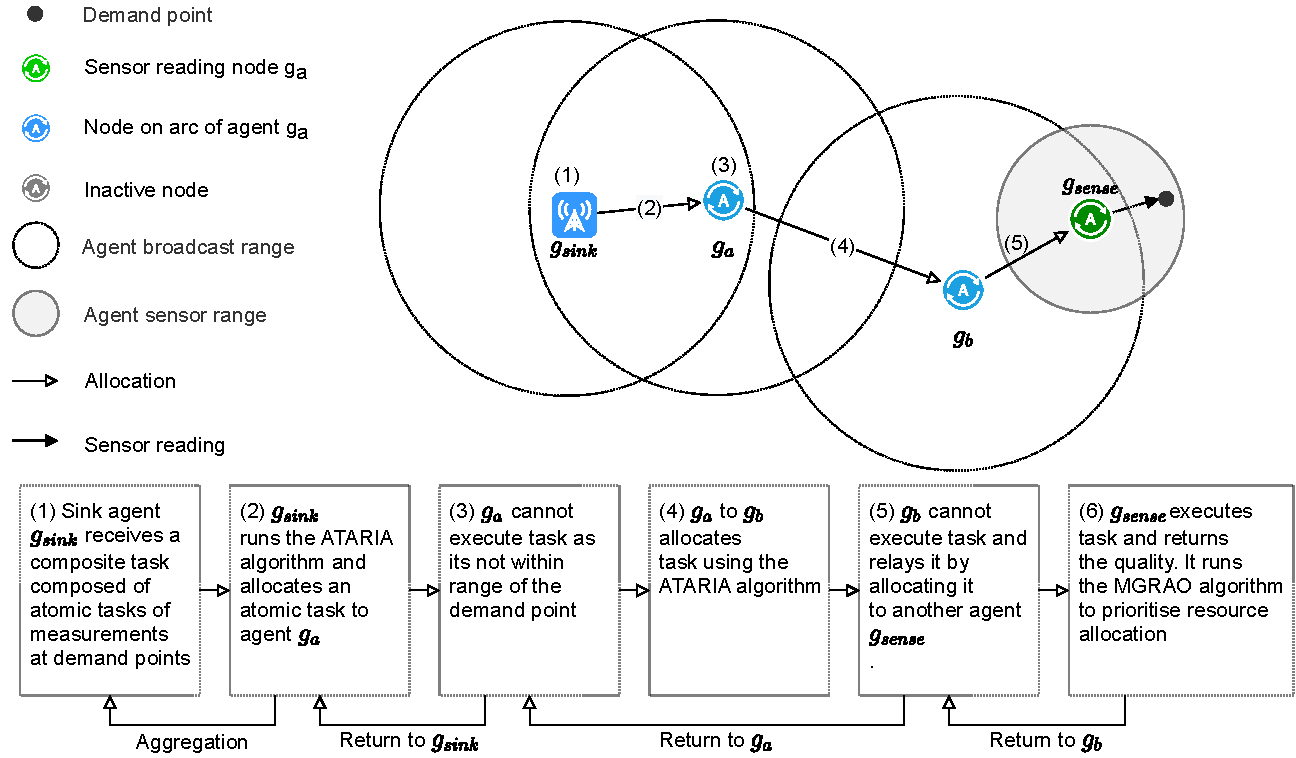
\includegraphics[width=0.8\linewidth, trim={25pt 0pt 25pt 0pt, clip}]{arc-flow}
	\caption{\textbf{Allocation along an arc}. This diagram illustrates how allocations can be relayed along an arc using successive applications of the \acronymATARIA{}{} algorithm.}
	\label{fig:arc-flow}
\end{figure}

The \acronymMGRAO{}{} algorithm helps agents executing atomic tasks allocate their resources to optimise the corresponding composite task value. This has two parts, an update algorithm that adjusts weights of resources based on received atomic task values, $\label{eq:mgrao_update}\formalMGRAOUpdate{}{}$,  and the application of these weights to generate the task execution quality itself, $\label{eq:mgrao_weighting}\formalMGRAOWeighting{}{}$. The update algorithm will change the resource weightings for an agent, $\functionAgentResources{}{}$, given the type of an atomic task completed, and the its absolute task value to the corresponding composite task. The weighting algorithm simply returns the resource weighting for calculation of an atomic tasks' quality $\functionAtomicTaskQualitySignature{}{}$ on its completion.


	\subsection{Configuration}

We simulated two systems to evaluate the algorithms in four different configurations (See Figure \ref{fig:system-types}).

\begin{figure}[ht]
	\centering
	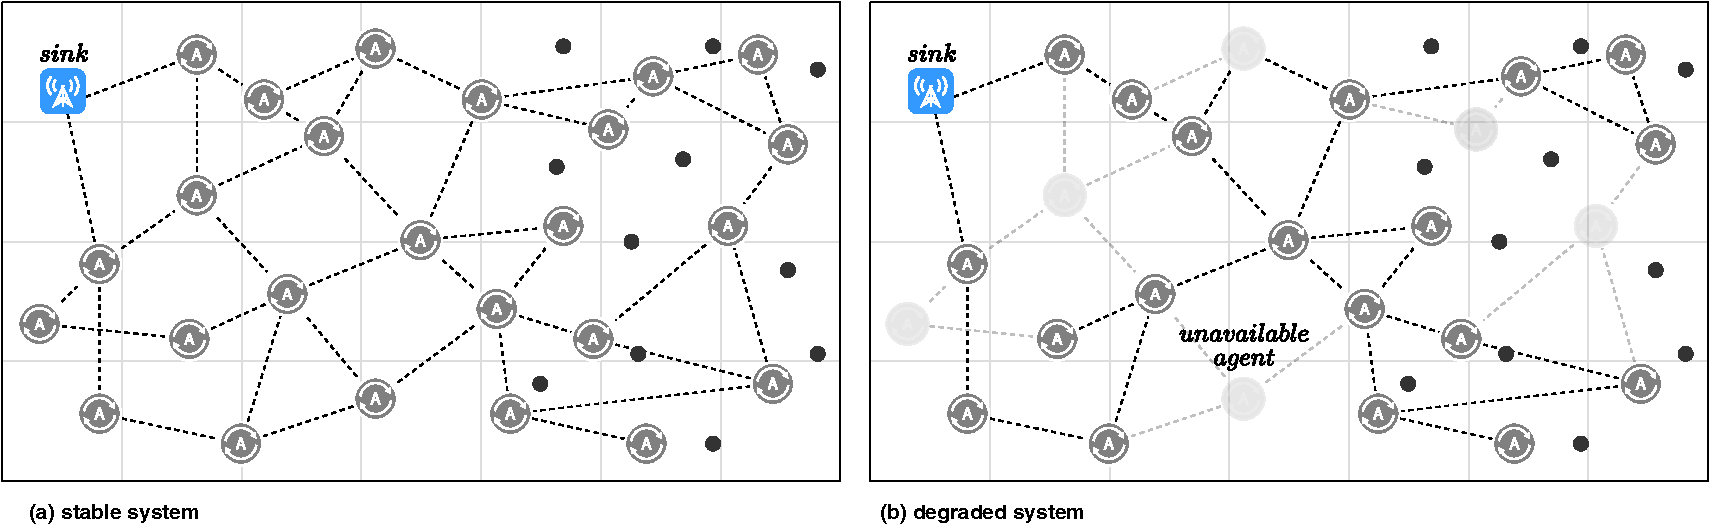
\includegraphics[width=0.9\linewidth]{system-types}
	\caption{\textbf{System types}. The diagram shows examples of the two systems. In the first \simulationSimple{}{}, there are $10$ possible agents that can execute the measurement task, tasks' demand points are distributed across the map. In the second, \simulationExtended{}{} system, there are $25$ agents that can execute the measurement tasks. The tasks' demand points are clustered away from the sink node.}
	\label{fig:system-types}
\end{figure}

The \simulationSimple{}{} system  equal weighting for each of the CTV components $\alpha, \beta, \gamma$ (Eq. \ref{eq:ctv}). The sink node was given $5$ measurement tasks to complete from outside the system, repeated $3$ times before one episode was complete. $10$ nodes were distributed randomly in the system, each capable of completing a task, or allocating it to any of $3$ nodes it was connected to. Each node could complete any measurement task with a quality dependent on their closeness to the demand point associated with the task (Eq. \ref{eq:atomic_task_quality}). The energy of all nodes in the system was fully reset at the end of each episode. An example of the simple system layout can be seen in Figure \ref{fig:system-types}(a). 

The \simulationExtended{}{} system had CTV component weightings where each of the relevant properties were given an $80\%$ dominance over the value of CTV value. The sink node was given $10$ measurements to allocate, with no repetition. It was also placed at a significantly large distance from the demand points associated with the tasks. $25$ nodes were distributed randomly in the system. This system examined the impact of the algorithm optimising the allocation of tasks towards the goals stated in Section \ref{section:optimisation_problem}. Task value could be maximised, but at the cost of longer arcs and therefore energy usage, or lower task values, and lower energy consumption. Figure \ref{fig:route_types} illustrates these two route types for task completion.

\subsection{Results}
Labels and descriptions for the algorithms are shown in Table \ref{table:summary_of_algorithms}, with configuration in Table \ref{table:summary_of_configurations}. Results for the \algorithmBalanced{}{} algorithm in the \simulationSimple{}{} system, and the \algorithmEnergy{}{}, \algorithmQuality{}{}, \algorithmDistribution{}{} algorithms in the \simulationExtended{}{} system are shown in Table \ref{table:results}.

System utility percentages show the summed values of composite tasks per episode (Eq. \label{eq:system_utility}) as compared to the theoretical maximum utility in the system \footnote{Note that the theoretical maximum is not necessarily attainable in all systems, dependent on their randomised node configurations.}. Energy available is presented as a percentage of that of a system containing nodes with full battery charge. We compare the different biases for optimisation across the CTV components of task values, energy availability, and distribution using quality-energy percentages. These use the available energy component in as a baseline, and show the percentage increase or decrease in average task qualities. Task-distribution shows the variation in the agents completing tasks, i.e. $\funcSize{set(\setAgents{}{})}{}/\funcSize{\setAgents{}{}}{}$. Higher values represent tasks being completed by distinct agents, with lower values meaning agents are completing multiple tasks. Arc depth data captures how many nodes re-allocated each task before completion.
	\section{Conclusions and future work}
\label{section:conclusions}

This work detailed and evaluated the \acronymWSNOptimisation{}{} algorithm and its application to wireless sensor network optimisation in dynamic and challenging environments. This is an extension of the previously described work on \acronymATARIA{}{} and \acronymMGRAO{}{} algorithms \citep{creech2021dynamic,creech2021resource} to hierarchical multi-agent systems. The algorithm was shown to optimise the and the quality of task completion and energy available in these systems, and to increase system lifetime through task and energy distribution. The algorithm was evaluated on a model WSN system based on a realistic situation where agents would be randomly distributed across a geographical area, where maintenance and management would be challenging due to harsh or dangerous conditions.  Our evaluation showed that the \acronymWSNOptimisation{}{} algorithm optimised the task quality, energy available, and distribution in the system as describe in Section \ref{section:experimental}, and that these components could be varied in their priorities through altering the $\alpha$, $\beta$ and $\gamma$ values of the CTV function (Section \ref{section:problem:optimising_resource_usage}, Eq. \ref{eq:taq}). This allowed the algorithm to balance across these different properties in the given systems and optimise for these multiple objectives in different ratios. 

Future work would look at implementing the algorithm in a larger scale network through simulation, as well as in the real-world, testing how the algorithm performs in a complex environment. There are a number of applications in WSN in which the agents involved are mobile. As the \acronymWSNOptimisation{}{} algorithm is designed to work in dynamic environments, where optimisation targets are non-stationary, we expect that it will also be useful in these types of system. Evaluation could be extended to simulations with mobile agents, and tested in real-world vehicle-to-vehicle communications (V2X) systems \citep{Gupta2017, Tong2019}. We also expect that testing practical deployment this work in the case of oceanographic monitoring would be a productive next step \citep{Albaladejo2010a}. The combination of harsh environmental conditions, difficulty of providing maintenance for remote agents, and mobility at slow speeds, should provide ideal conditions for successful use of \acronymWSNOptimisation{}{}.


  
	\printcredits

%% Loading bibliography style file
%\bibliographystyle{model1-num-names}
\bibliographystyle{cas-model2-names}

% Loading bibliography database
\bibliography{cas-refs}

	%\vskip3pt

\bio{figs/niall}
Author biography without author photo.
Author biography. Author biography. Author biography.
Author biography. Author biography. Author biography.
Author biography. Author biography. Author biography.
Author biography. Author biography. Author biography.
Author biography. Author biography. Author biography.
Author biography. Author biography. Author biography.
Author biography. Author biography. Author biography.
Author biography. Author biography. Author biography.
Author biography. Author biography. Author biography.
\endbio

\bio{figs/natalia}
Author biography with author photo.
Author biography. Author biography. Author biography.
Author biography. Author biography. Author biography.
Author biography. Author biography. Author biography.
Author biography. Author biography. Author biography.
Author biography. Author biography. Author biography.
Author biography. Author biography. Author biography.
Author biography. Author biography. Author biography.
Author biography. Author biography. Author biography.
Author biography. Author biography. Author biography.
\endbio

\bio{figs/simon}
Author biography with author photo.
Author biography. Author biography. Author biography.
Author biography. Author biography. Author biography.
Author biography. Author biography. Author biography.
Author biography. Author biography. Author biography.
\endbio
	\begin{appendix}
	\section{Symbols}

\begin{table}[pos=htp]
	\begin{tabular}{|p{0.1\textwidth}|p{0.3\textwidth}|p{0.5\textwidth}|}
		\hline
		Symbol & Name & Definition \\
		\hline
		$\varTime{}{}$ & System time & XXX \\
		$\varAtomicTask{}{}$ & Atomic task & XXX \\
		$\varCompositeTask{}{}$ & Composite task & XXX \\
		$\varAgent{}{}$ & Agent & XXX \\
		$\varIdleAgent{}{}$ & Agent (idle mode) & XXX \\
		$\varSleepAgent{}{}$ & Agent (sleep mode) & XXX \\
		$\varChildAgent{}{}$ & Child agent & XXX \\
		$\varParentAgent{}{}$ & Parent agent & XXX \\
		\hline
	\end{tabular}
	\caption{Notation for agents}
\end{table}

\begin{table}[pos=htp]
	\begin{tabular}{|p{0.1\textwidth}|p{0.3\textwidth}|p{0.5\textwidth}|}
		\hline
		Symbol & Name & Definition \\
		\hline
		$\varOrchestrationEnergy{}{}$ & Orchestration energy & XXX \\
		$\varTransmissionEnergy{}{}$ & Transmission energy & XXX \\
		$\varReceiverEnergy{}{}$ & Receiver energy & XXX \\
		$\varSleepEnergy{}{}$ & Sleep mode energy & XXX \\
		$\varIdleEnergy{}{}$ & Idle mode energy & XXX \\
		$\functionSystemEnergyConsumption{}{}$ & System energy consumption& XXX \\
		$\functionTaskEnergy{}{}$ & Task energy consumption & XXX \\
		$\functionSystemEnergyVariability{}{}$ & System energy variability& XXX \\
		$\functionAgentEnergyAvailable{}{}$ & Agent energy available & XXX \\
		$\functionAgentEnergyTotal{}{}$ & Agent energy total & XXX \\
		$\functionSystemEnergyAvailable{}{}$ & System energy available & XXX \\
		$\varBatteryEnergy{}{}$ & Battery energy & XXX \\
		$\varBatteryEnergyMax{}{}$ & Maximum battery energy & XXX \\
		\hline
	\end{tabular}
	\caption{Notation for energy}
\end{table}

\begin{table}[pos=htp]
	\begin{tabular}{|p{0.1\textwidth}|p{0.3\textwidth}|p{0.5\textwidth}|}
		\hline
		Symbol & Name & Definition \\
		\hline
		$\functionProbabilityInit{}{}$ & Initial failure probability & XXX \\
		$\functionProbabilityRand{}{}$ & Random failure probability & XXX \\
		$\functionProbabilityWear{}{}$ & Wear-out failure probability & XXX \\
		$\functionProbabilityFail{}{}$ & Overall failure probability & XXX \\
		$\varConstantInit{}{}$ & Max initial failure probability & XXX \\
		$\varConstantRand{}{}$ & Max random failure probability & XXX \\
		$\varConstantWear{}{}$ & Max wear-out failure probability & XXX \\
		$\varEnergyInit{}{}$ & Initial failure threshold energy & XXX \\
		$\varEnergyWear{}{}$ & Wear-out failure threshold energy & XXX \\
		$\functionCompositeTaskCoverage{}{}$ & Composite task coverage & XXX \\
		\hline
	\end{tabular}
	\caption{Notation for lifecycle}
\end{table}

\begin{table}[pos=htp]
	\begin{tabular}{|p{0.1\textwidth}|p{0.3\textwidth}|p{0.5\textwidth}|}
		\hline
		Symbol & Name & Definition \\
		\hline
		$XXX$ & XXX & XXX \\
		\hline
	\end{tabular}
	\caption{Notation for location}
\end{table}
	\todo[inline]{PROBLEM - LIFECYCLE}
\subsubsection{Sensor lifetime in WSN}
We can model the failure of nodes through a simple bathtub model as described by the three phases of node lifespan as seen in Figure \ref{fig:node_reliability_lifespan},
\begin{figure}
	\centering
	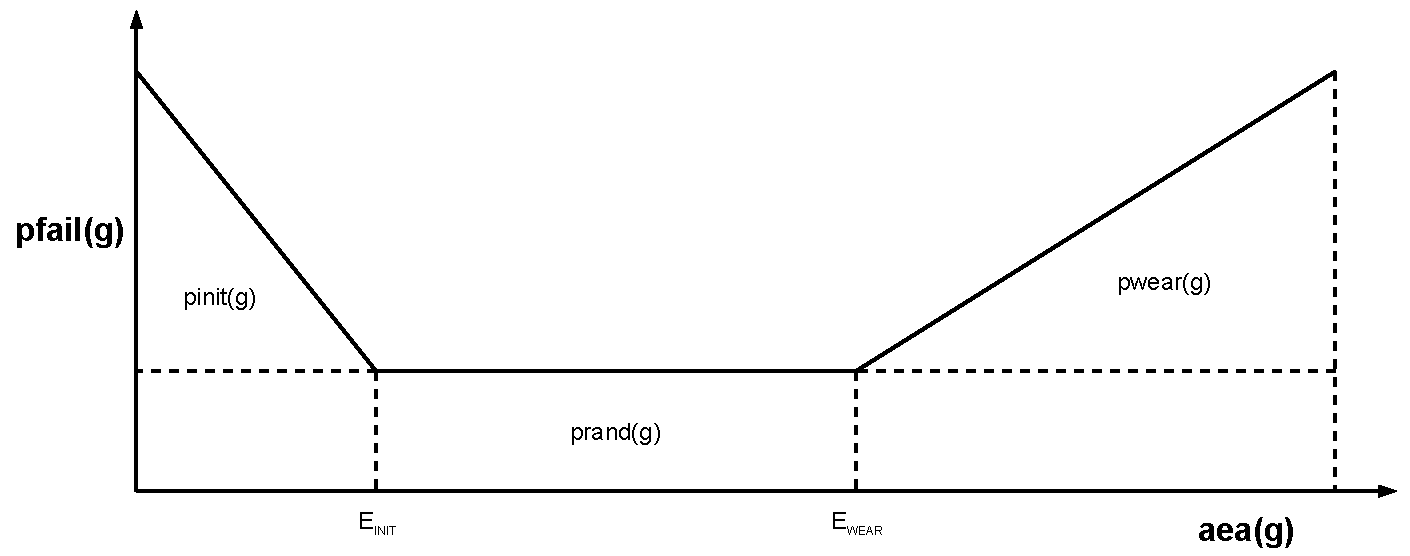
\includegraphics[width=0.7\linewidth]{node_reliability_lifespan}
	\caption[Probability of failure with lifetime energy usage for a node]{Probability of failure with lifetime energy usage for a node}
	\label{fig:node_reliability_lifespan}
\end{figure}
\begin{enumerate}
	\item $\functionProbabilityInit{}{}$, the initial failure probability, component failures early in lifespan, decreasing with time.
	\item $\functionProbabilityRand{}{}$, the random failure probability, the constant background failure rate.
	\item $\functionProbabilityWear{}{}$, the wear-out failure probability, the increasing failure rate towards the end of a nodes expected lifespan.
\end{enumerate}
For each node, we use $\functionAgentEnergyTotal{}{}$ as a proxy for time so the probability of an agent $\varAgent{}{}$ having a permanent failure increases with usage.

\definition[Probability of node failure]{
	The probability of node failure for an agent $\varAgent{}{}$ is $\functionProbabilityFail{}{}$, the combination of the probabilities of initial, random, and wear-out failures given the agents total energy usage in its lifetime $\functionAgentEnergyTotal{}{}$.
	\begin{equation}
		\functionProbabilityFail{}{} = \underbrace{max(0, (1 - \functionAgentEnergyTotal{}{}/\varEnergyInit{}{})) \times \varConstantInit{}{}}_{\functionProbabilityInit{}{}} + \underbrace{\varConstantRand{}{}}_{\functionProbabilityRand{}{}} + \underbrace{max(0, ( \functionAgentEnergyTotal{}{}/\varEnergyWear{}{}))\times \varConstantWear{}{}}_{\functionProbabilityWear{}{}}
	\end{equation}
	Where $\varEnergyInit{}{}{}{}$ is the energy level where initial failures are effectively zero,  and $\varEnergyWear{}{}{}{}$ where wear-out failures become a factor. $\varConstantInit{}{}$, $\varConstantRand{}{}$, and $\varConstantWear{}{}$  are constants chosen to scale the effects of initial failures and wear-out failures respectively.
}




	%\subsubsection{Energy recovery}

%%%%%%%%%%%%%%%%%% NOTATION %%%%%%%%%%%%%%%%%%%%%%%%%%
\newcommand{\setEnergyDeltaIdle}[2]{\Delta\setSymbol{E}{\texttt{idle}}{#2}}
\newcommand{\setEnergyHarvest}[2]{\setSymbol{E}{\texttt{harvest}}{#2}}
\newcommand{\setEnergyWUR}[2]{\setSymbol{E}{\texttt{idle-wur}}{#2}}
%%%%%%%%%%%%%%%%%%%%%%%%%%%%%%%%%%%%%%%%%%%%%%%%%%%%%%

When not sampling, aggregating, or broadcasting a node recovers energy at a rate given by the energy harvesting solar panel minus that lost by having the WUR in standby.

\begin{equation}
	\setEnergyDeltaIdle{}{}
	= 
	\setEnergyHarvest{}{}
	-
	\setEnergyWUR{}{}
\end{equation}



	\end{appendix}
				
\end{document}
			
